\documentclass[a4paper, twocolumn]{article}

%% Margins
\usepackage[hmargin=1.8cm, vmargin=3cm]{geometry}
\setlength{\columnsep}{0.6cm}

%% Fonts
\usepackage{libertine}
\usepackage{libertinust1math}
\usepackage[T1]{fontenc}

\usepackage{scrextend}
\changefontsizes[11.5pt]{9.5pt}

%% Section styles
\makeatletter
\renewcommand{\subsection}{\@startsection{subsection}{2}{\z@}%
                                     {-3.25ex\@plus -1ex \@minus -.2ex}%
                                     {1.5ex \@plus .2ex}%
                                     {\normalfont\normalsize\bfseries}}
\makeatother

%% Figures and tables
\usepackage{graphicx}
\graphicspath{{./figures/}}
\usepackage{caption}
\belowcaptionskip=0.5cm

%% Re-numbering supplementary figures and tables
\newcommand{\beginsupplement}{%
        \setcounter{table}{0}
        \renewcommand{\thetable}{S\arabic{table}}%
        \setcounter{figure}{0}
        \renewcommand{\thefigure}{S\arabic{figure}}%
        }

%% References
\usepackage{cite}

%% Symbols
\usepackage{gensymb}

%% Japanese
\usepackage{CJKutf8}
\newcommand*{\ja}[1]{%
  \begin{CJK}{UTF8}{ipxm}#1\end{CJK}}

%=====================================


\begin{document}
\onecolumn
\thispagestyle{empty}
\begin{center}
\vspace{0.5cm}

{\Large
Department of Computational Biology and Medical Sciences

\vspace{0.2cm}

Graduate School of Frontier Sciences

\vspace{0.3cm}

The University of Tokyo
}

\vspace{1cm}

{\huge 2016}

\vspace{1cm}

{\Large Master's Thesis}

\vspace{3cm}

{\huge Centromeric sequence organization in medaka}

\vspace{2.5cm}

{\huge Shingo Tomioka}

\vspace{3cm}

{\Large Supervised by}

\vspace{0.3cm}

{\Large Professor Shinichi Morishita}

\vspace{4cm}

{\Large Submitted January 27, 2017}


\end{center}

\addtocounter{page}{-1}

%\section*{Abstract}

\fontdimen2\font=0.3em  % word spacing
\twocolumn

\section*{Introduction}
\subsection*{The centromere}
  The centromere is a chromosomal region where kinetochore forms and plays a critical role for proper chromosome segregation in mitosis and meiosis. The centromere is characterized by the presence of centromere-specific histone H3 variant CENH3 (also known as CENP-A). In the majority of species studied so far, the centromere is comprised of repetitive DNA \cite{Plohl2014}. Despite its fundamental biological importance, the mechanism how the position of the centromere is specified are still insufficiently understood \cite{McKinley2016}.


\subsection*{DNA sequences at the centromere}
  Repeat-based centromere is the most common structure in eukaryote species \cite{Plohl2014}. One of the major components of the repeat-based centromeres is a tandemly-repeated satellite DNA. Despite the conserved biological function of the centromere, DNA sequences at the centromere evolves rapidly (known as ``centromere paradox'') and the satellite sequences are generally species-specific \cite{Henikoff2001}. A well-known example is a 171-bp AT-rich alpha-satellite observed in human and many other primate species \cite{Willard1991}. In the human genome, tandemly-repeated alpha-satellites comprise hundred kilobase- to megabase-sized arrays in each chromosome \cite{Willard1987}. The satellite DNA can be highly diverged within a species, whereas the inner centromeric regions tend to have highly homogenous repeat arrays. In many primate species including human, the core centromeres consist of higher-order repeats (HORs) where several alpha-satellite monomers comprise a repeat unit which itself iterates tandemly with extremely high identity ($>$95\%) \cite{Willard1987}. Another major component of the repeat-based centromeres is retrotransposons, which has been widely observed in plant species \cite{Wang2009, Lermontova2015}. Satellites and retrotransposons are not mutually exclusive, rather intermingled structure of them are commonly observed \cite{Plohl2014}. These regional centromeres are flanked by heterochromatic pericentromeres. Centromeres and pericentromeres are characterized by distinct chromatin structures which are regulated by different epigenetic marks \cite{Verdaasdonk2011, McKinley2016}.

  While repeat-based regional centromeres are the most common structure in eukaryotes, some species have different types of centromeres. Budding yeast \textit{Saccharomyces cerevisiae} has a ``point centromere'' where $\sim$125-bp specific sequences form centromeres. In nematode \textit{C. elegans} and some insects and plants, the spindle microtubules attach all along a chromosome and the entire chromosome functions as a centromere, called ``holocentromere'' \cite{Plohl2014, Fukagawa2014}.

  % TODO: add reference of budding yeast centromere


\subsection*{Centromere specification and role of underlying DNA sequences}
  Understanding the machinery of centromere formation is still ongoing challenge \cite{Plohl2014, Fukagawa2014, McKinley2016}. The chromosomal position where the centromere forms is believed to be specified by the cooperation of centromere-specific histone variant CENP-A, histone modifications and underlying DNA sequences \cite{Fukagawa2014}. However, specific DNA sequences are not considered to be indispensable for the centromere formation, which is inferred by the observations of several ``atypical'' centromeres.

  Neocentromeres are the centromeres that form on ectopic sites distantly from original centromeres along with a loss or an inactivation of the original ones and have been widely observed in many species \cite{Marshall2008, Scott2014}. Neocentromeres can form on loci that do not have repetitive sequences or specific sequence motifs. Dicentric chromosomes have also been widely observed, which possess two regions with centromeric sequences and one of them directs the centromere formation whereas the other one remains inactivated \cite{Earnshaw1985, Steiner1994, Han2006}. It is also known that some species have a few chromosomes with repeat-free centromeres among the other chromosomes with repeat-based centromeres \cite{Piras2010, Shang2010, Locke2011}.

  The wide prevalence of repetitive DNA among eukaryote species despite these seeming dispensability for centromere formation suggest that repetitive DNA may stabilize the centromere, rather than specify its formation. Some researchers have proposed that the repetitive DNA may serve as a wide range of ``safe'' region without genes thus provide plasticity for obscure positions of kinetochore formation \cite{Plohl2014, Fukagawa2014}. It has been hypothesized that tandem repeats occur spontaneously at any genomic position and amplify by unequal crossover between sister chromatids, homologous chromosomes and non-homologous chromosomes \cite{Smith1976, Willard1991, Charlesworth1994}; therefore the naturally-expanded repetitive regions may be selected as a suitable ``safe'' region for the centromere formation. Moreover, the neocentromeres and repeat-free centromeres may be premature forms that will gradually acquire repetitive DNA \cite{Fukagawa2014}. On the other hand, the presence of a widely-conserved $\sim$17-bp sequence motif (CENP-B box) and several recent functional studies \cite{Henikoff2015, Aldrup-MacDonald2016} imply more direct contribution of the underlying DNA sequences to the centromere formation.


\subsection*{Early studies}
  Fundamental understanding of centromeric sequence characteristics was established by a number of early studies in 1980's and 1990's, mainly targeting human centromeres. These studies based on experimental methods such as genomic fragmentation by restriction enzymes, pulsed field gel electrophoresis and DNA hybridization.

  The findings include approximate estimation of repeat array size and its divergence among individuals \cite{Oakey1990, Mahtani1990, Greig1991}, the presence of chromosome-specific alpha-satellite HORs \cite{Willard1987} and super-chromosomal subfamilies of alpha-satellites \cite{Alexandrov1988, Alexandrov2001}. It was also revealed that alpha-satellite is widely shared within primate species and even HOR patterns are shared with closely-related species including chimpanzee, gorilla and orangutan \cite{Willard1991}.


\subsection*{The genome projects era}
  Although the basic characteristics of centromeric sequences were revealed by these early studies, understanding detailed sequence organization of the centromere has been challenging in many species, due to the difficulty of assembling its highly-repetitive sequences. In the human genome project, which declared its completion in 2003, large portion of centromeric sequences were missed as huge gaps. Whereas divergent monomeric portion around pericentromeres were assembled in many chromosomes, the assemblies reached more homogeneous HOR regions in a limited number of chromosomes \cite{M.KatharineRuddand2004, She2004}. Nevertheless, subsequent analyses on these few chromosomes revealed sequence landscapes with never-seen resolution \cite{Schueler2001, Ross2005, Nusbaum2006, Rudd2006}. The poor sequence assembly at the repetitive centromeric regions were the case in other contemporarily-assembled species \cite {Waterston2002, Hoskins2007}.


\subsection*{Second-generation sequencing-based studies}
  Although second-generation sequencers (SGSs) represented by Illumina and 454 accomplished a number of genome assemblies \cite{Schatz2010}, they achieved virtually no improvement in centromeric sequence assembly because of their short read length, emphasizing that centromere studies need specific approaches considering its sequence characteristics. Nonetheless, their high throughput sequencing combined with chromatin immunoprecipitation (ChIP-seq) facilitated identification of centromere-associated sequences in many species \cite{} and characterization of functional regions in the assembled centromeric sequences \cite{Hayden2013}.


\subsection*{Computational studies}
  A number of computational studies on centromeric sequences were conducted using Sanger and Illumina whole genome shotgun (WGS) sequencing data, some of which made remarkable achievement. Some studies identified candidate centromeric satellite sequences from WGS data \cite{Alkan2011, Melters2013}, whereas others identified novel HOR patterns from assembled sequences \cite{Rosandic2003} or from WGS data \cite{Alkan2007}.

  Melters \textit{et al}. \cite{Melters2013} identified candidate centromeric satellite sequences of 282 species (204 animal and 78 plant species) using WGS data from various sequencing platforms, mainly from Sanger and Illumina. They based on the assumption that the most abundant tandem repeat in a genome derives from centromeric sequences, which is true for most species whose centromeric sequences has been previously characterized. This study revealed that centromeric satellites from various eukaryotic species do not share common properties such as repeat unit length, GC content or genomic abundance and that centromeric satellite sequences are conserved among only closely-related species of within 50 million years after separation. These results confirmed a traditional view that centromeric sequences evolves rapidly, independently of the rest of genomic sequences \cite{Henikoff2001}.

  Another remarkable computational study is from Miga \textit{et al}. \cite{Miga2014}, in which they generated centromeric array sequences of each human chromosome, using graph-based probabilistic models constructed from Sanger WGS reads. Although the generated sequences do not guarantee long-range ordering of the satellite sequences, they adequately represent local ordering, thus provide useful scaffolds for mapping sequencing reads and/or other downstream analyses. The generated centromeric sequences, moreover, has been included in the latest human reference genome (GRCh38) \cite{GenomeRef2013}.


\subsection*{Feasibility of long-read sequencing}
  Despite these development in sequencing technologies and computational methods, long-range organization of centromeric sequences could not be resolved mainly due to the short read length of Sanger or SGS technologies. However, recently-emerging long-read technologies of PacBio \cite{Eid2009} and Oxford Nanopore \cite{Jain2016} are expected as promising tools for centromere studies \cite{Aldrup-MacDonald2014, Miga2015}.

  PacBio single-molecule real-time (SMRT) sequencing yields average read length of $\sim$15kb and longest of $\sim$50kb with P6-C4 chemistry. This long read length enables to capture long-range structure such as HORs directly and provides more opportunity to anchor repetitive sequences to adjacent unique regions. Although error rate of PacBio sequencing is relatively high ($\sim$15\%), the error pattern is believed to be completely random, thus can be successfully corrected with enough sequencing coverage \cite{Myers2014}. Furthermore, in contrast to Sanger or SGS technologies which suffer from sequencing bias deriving from PCR amplification and/or vector cloning steps, amplification-free PacBio sequencing involves no apparent sequencing bias \cite{Ross2013}. In recent years, a number of studies have reported dramatic improvement in genome assemblies using PacBio sequencing, some of which improved centromere assembly as well \cite{VanBuren2015, Vij2016, Jiao2016}. Among these, a \textit{de novo} assembly of a grass genome covered three of the nine centromeric regions which are comprised mainly of 155-bp satellite sequences and spans $\sim$400 kb \cite{VanBuren2015}. Some studies targeting centromere-associated repeat-rich regions have also been conducted with PacBio sequencing \cite{Wolfgruber2016, Khost2016}, and a computational tool for detecting HOR patterns from long reads was also developed \cite{Sevim2016}.

  % TODO: add references of PacBio-based assemblies

  Oxford Nanopore sequencing yields even longer read length (e.g. MinION sequencer routinely yields $>$150 kb read) with accuracy of $\sim$92\% \cite{Jain2016}. However, some early-adopting laboratories of it including the author's laboratory observe unstable read length and much higher error rate than the officially announced rate (Kin Fai Au, personal communication), thus the community awaits improvement and sophistication of its sequencing technology and protocols.


\subsection*{Limited number of in-depth studies, especially in fish species}
  Due to the long-standing difficulty in assembling centromeric regions, in-depth analysis of centromeric sequences have been conducted in a limited number of species, including human, some other primates, mouse, some plants, \textit{Drosophila} and yeasts, and scarce in fish species. Centromere-associated satellites have been identified or confirmed in zebrafish, seabass and stickleback by CENP-A-targeted ChIP and/or FISH experiments \cite{Phillips2000, Kuznetsova2014, Cech2015}, however only limited amount of them have been included in the assembled genomes \cite{Howe2013, Vij2016, Cech2015}. Medaka, as well as zebrafish, has traditionally played an important role as a model organism of fish species \cite{Wittbrodt2002}. Cloning-based assembly of its genome was conducted about ten years ago \cite{Kasahara2007}, however centromeric regions were largely missed in gaps, as was the case in many contemporary assembly projects. A 156-bp candidate centromeric satellite sequence of medaka was identified in a computational study by Melters \textit{et al} \cite{Melters2013}, though whether this sequence truly derives from the centromere has not been confirmed by experimental methods such as ChIP-seq or FISH.


\subsection*{This study}
  The author's laboratory recently assembled three medaka inbred strain genomes using PacBio long reads and achieved dramatic improvement in the assembly quality (Ichikawa \textit{et al.}, unpublished). Based on these high quality medaka genomes, this study conducted in-depth analysis of medaka centromeric sequences. This study revealed the presence of inter-chromosomal relationship of the satellite sequences and its conservation among the strains. Also the evidence of higher-order structure (HORs) was captured.


\section*{Results}
\subsection*{Genome assembly of three medaka strains}
  Three medaka inbred strains were recently sequenced with PacBio single-molecule real-time (SMRT) sequencing and were assembled by the author's laboratory (Ichikawa \textit{et al}., unpublished; see Methods for an overview of the assembly procedure). Two strains (Hd-rR and HNI) were established from northern and southern Japanese populations, respectively and the other one (HSOK) was from eastern Korean population. The two Japanese populations are estimated to have separated 18 million years ago (MYA), whereas the ancestor of the two Japanese populations and that of the eastern Korean population are estimated to have separated 25 MYA \cite{Setiamarga2009}.


\subsection*{Genomic abundance of centromeric repeats}
  This study started with a candidate centromeric satellite sequence of medaka which was identified in a previous computational study \cite{Melters2013}. In that study, Melters \textit{et al.} estimated that the candidate centromeric satellite comprise 0.32\% of the medaka genome. However this estimation can underestimate the true genomic abundance due to its identification strategy. In order to better infer the genomic abundance of the centromeric satellite, PacBio raw reads were searched for the centromeric satellite sequence.

  Genomic fraction of the centromeric repeat was estimated by searching PacBio subreads for the representative monomer sequence with RepeatMasker \cite{Smit}. The genomic fraction in Hd-rR and HNI genomes were estimated to be $\sim$1\%, while that in the HSOK genome was $\sim$2\% (Table \ref{centromeric_repeat_genomic_abundance}). This difference is consistent with the previous observations that centromeric repeat array size in a chromosome can vary up to 20-fold among individuals within a species \cite{Miga2014}. Assuming the genome size to be 800 Mb, the centromeric satellite comprise 8--16 Mb of the genome, which implies each chromosome has around 500 kb of centromeric satellite on average. This is concordant with the observations that the centromere of many higher eukaryotes studied to date are characterized by hundreds to thousands of kilobases of satellite sequences \cite{Plohl2014}. Although quantifying the centromeric satellite in erroneous PacBio reads can lead to slight underestimation, the estimation should be more reliable than the clustering-based estimation using short Sanger reads in the previous study \cite{Melters2013}.


\subsection*{Centromeric repeat distribution}
  The distribution of the centromeric satellites in the three medaka genomes was investigated. The three assembled genomes were searched for the candidate centromeric satellite sequences using RepeatMasker (Table\,\ref{centromeric_repeat_distribution}, Fig.\,\ref{fig:repeat_distribution}). The results revealed that all the identified centromeric satellite arrays were truncated by contig gaps at either or both ends, suggesting none of the centromeric regions was spanned by a single contig. In the Hd-rR and HSOK genomes, $\sim$1-Mb centromeric satellites were identified in total, respectively, whereas only $\sim$80\,kb was identified in the HNI genome. This substantial difference in the amounts of identified centromeric satellite is presumably due to the difference in read length. The HSOK genome was sequenced with the newest P6-C4 chemistry and the average read length was 11\,kb; Hd-rR was sequenced with the combination of P6-C4 and older P5-C3 and P4-C2 chemistries and the average read length was 6.5\,kb; HNI was sequenced with P5-C3 and P4-C2 with the average read length of 3.6\,kb (Table\,\ref{sequencing_stats}). In addition, substantial amount of the centromeric satellite was identified in the contigs that failed to anchor to the chromosomes. The enrichment of identified centromeric satellite in unanchored contigs to in anchored contigs was as big as 12-fold in HSOK and 27-fold in HNI, in contrast to relatively small 3-fold enrichment in Hd-rR (Table\,\ref{centromeric_repeat_distribution}). In the Hd-rR genome assembly, contigs were scaffolded using BAC-/Fosmid-end sequencing reads and Hi-C contact frequency data, which successfully anchored a number of contigs containing centromeric satellites, emphasizing the effectiveness of complementing the long-read sequencing with other methods that capture even longer-range information.

  % TODO: describe that sum of satellites in the anchored and unanchored contigs did not reach the estimated abundance.

  For those chromosomes that have $>$1 kb centromeric repeat, positions of the centromeres in chromosomes were classified into metacentric, submetacentric, subtelocentric and acrocentric, employing the nomenclature by Levan \textit{et al.} \cite{levan1964} (Table\,\ref{centromeric_repeat_distribution}). Although this nomenclature originally based on karyotype observation rather than DNA sequence level and the positions induced from the two levels can slightly differ, the sequence-based classification conducted here is  nevertheless informative for interpreting subsequent analyses. The number of chromosomes classified to each type was in line with previous karyotype studies \cite{Uwa1981, Uwa1990}.

  Centromeric positions of the same chromosome were mostly conserved among the strains, confirmed by observing the corresponding pair of genetic markers flanked the repeat arrays, with only two exceptions in chromosomes 4 and 6 (Fig. \ref{fig:repeat_distribution}). For chromosome 4, Hd-rR had an acrocentric repeat array, whereas HSOK had a metacentric array. For chromosome 6, all the three strains had acrocentric repeat arrays but those of Hd-rR and HSOK and that of HNI located on the opposite end of the chromosome. As the karyotype study has revealed that the three strains possess slightly different sets of centromeric positions \cite{Uwa1990}, the difference of chromosomes 4 and 6 may be derived from \textit{bona fide} karyotype difference. Notably, Hd-rR chromosome 21 possessed metacentric and acrocentric arrays of nearly the same length (41.6 kb and 45.5 kb, respectively; Fig. \ref{fig:repeat_distribution}), thus this chromosome may dicentric where one of the arrays forms the functional centromere whereas the other is silenced.

  \begin{table*}[htp]
    \centering
    \caption{Centromeric repeat distribution}
    \begin{tabular}{r|rc|rc|rc}
  \hline
  & \multicolumn{2}{c|}{Hd-rR} & \multicolumn{2}{c|}{HNI} & \multicolumn{2}{c}{HSOK} \\ \hline
  chromosome & total repeat (bp) & position & total repeat (bp) & position & total repeat (bp) & position \\ \hline
  1  & 48,805  & SM  & 0      & -  & 0       & -  \\
  2  & 54,844  & M   & 3,831  & M  & 64,213  & M  \\
  3  & 52,681  & ST  & 0      & -  & 0       & -  \\
  4  & 10,513  & A   & 0      & -  & 305,521 & M  \\
  5  & 0       & -   & 10,605 & A  & 0       & -  \\
  6  & 8,226   & A   & 1,635  & A  & 7,020   & A  \\
  7  & 0       & -   & 12,911 & A  & 25,917  & A  \\
  8  & 59,863  & SM  & 0      & -  & 324,346 & SM \\
  9  & 40,159  & SM  & 0      & -  & 0       & -  \\
  10 & 0       & -   & 14,685 & ST & 0       & -  \\
  11 & 4,755   & A   & 4,513  & A  & 66,412  & A  \\
  12 & 232,280 & SM  & 25,683 & SM & 40,516  & SM \\
  13 & 35,778  & A   & 0      & -  & 0       & -  \\
  14 & 33,284  & A   & 0      & -  & 0       & -  \\
  15 & 0       & -   & 0      & -  & 63,112  & A  \\
  16 & 12,804  & A   & 0      & -  & 0       & -  \\
  17 & 1,588   & A   & 0      & -  & 0       & -  \\
  18 & 23,853  & SM  & 0      & -  & 9,236   & SM \\
  19 & 131,040 & SM  & 4,830  & SM & 4,757   & SM \\
  20 & 96,309  & ST  & 0      & -  & 17,574  & ST \\
  21 & 87,124  & M/A & 2,131  & A  & 0       & -  \\
  22 & 61,066  & A   & 0      & -  & 4,942   & A  \\
  23 & 6,580   & M   & 0      & -  & 25,847  & SM \\
  24 & 0       & -   & 0      & -  & 0       & -  \\
  \hline
  anchored total & 1,001,552 &  & 80,824 &  & 959,413 \\
  unanchored total & 3,279,256 & (5.89\%) & 2,254,882 & (3.16\%) & 11,273,168 & (17.5\%) \\
  total & 4,280,808 &  & 2,335,706 &  & 12,232,581 \\
  \hline
  positions summary & \multicolumn{2}{c|}{2M+6SM+2ST+8A (6U)} & \multicolumn{2}{c|}{1M+2SM+1ST+5A (15U)} & \multicolumn{2}{c}{2M+5SM+1ST+5A (11U)} &
  \hline
\end{tabular}

    \label{centromeric_repeat_distribution}
    \caption*{{\small
      Total amount of the centromeric repeats identified in the chromosomes are shown. The total amount in the contigs that were anchored to the chromosomes and in the unanchored contigs are also shown (fraction of the centromeric repeats in the unanchored contigs are shown in the brackets). The centromeric positions were determined by the repeat distribution on each chromosome, employing the nomenclature by Levan \textit{et al.} \cite{levan1964}. Hd-rR chromosome 21 possessed centromeric repeat arrays of nearly the same length (41.6 kb and 45.5 kb) at the positions corresponding to metacentric and acrocentric, thus described as 'M/A'. M, metacentric; SM, submetacentric; ST, subtelocentric; A, acrocentric; U, unknown (due to the lack of centromeric repeats).
    }}
  \end{table*}


\subsection*{Centromeric sequence mapping by FISH}
  To confirm that the candidate centromeric satellite sequence truly localizes to the centromeres, FISH experiment was conducted. Probe sequences were designed by the author and the FISH experiments were carried out by a collaborator (see Methods).

  The candidate satellite identified by Melters \textit{et al.} \cite{Melters2013} was first used as a hybridization probe and signals were observed only from 5$\sim$7 chromosome pairs (Fig.\,\ref{fish_each}). In order to map the centromeres of the other chromosomes, additional probes were designed (see Methods). The additional probes successfully hybridized to some chromosomes that the first probe failed to hybridize, with approximately the same positions as expected by the \textit{in silico} centromeric repeat distribution (Fig.\,\ref{fish_each}, Table\,\ref{centromeric_repeat_distribution}), although two additional probes hybridized to less chromosomes than expected by the \textit{in silico} alignment results. When all the probes combined, signals were observed at the centromeres of $\sim$13 pairs of chromosomes (Fig.\,\ref{fish_all}). This result confirmed that the candidate centromeric satellite truly derives from the centromeres. Moreover, the number of the chromosomes having each centromeric positions were largely consistent with the sequence-based results in the previous section.

  \begin{figure*}
    \centering
    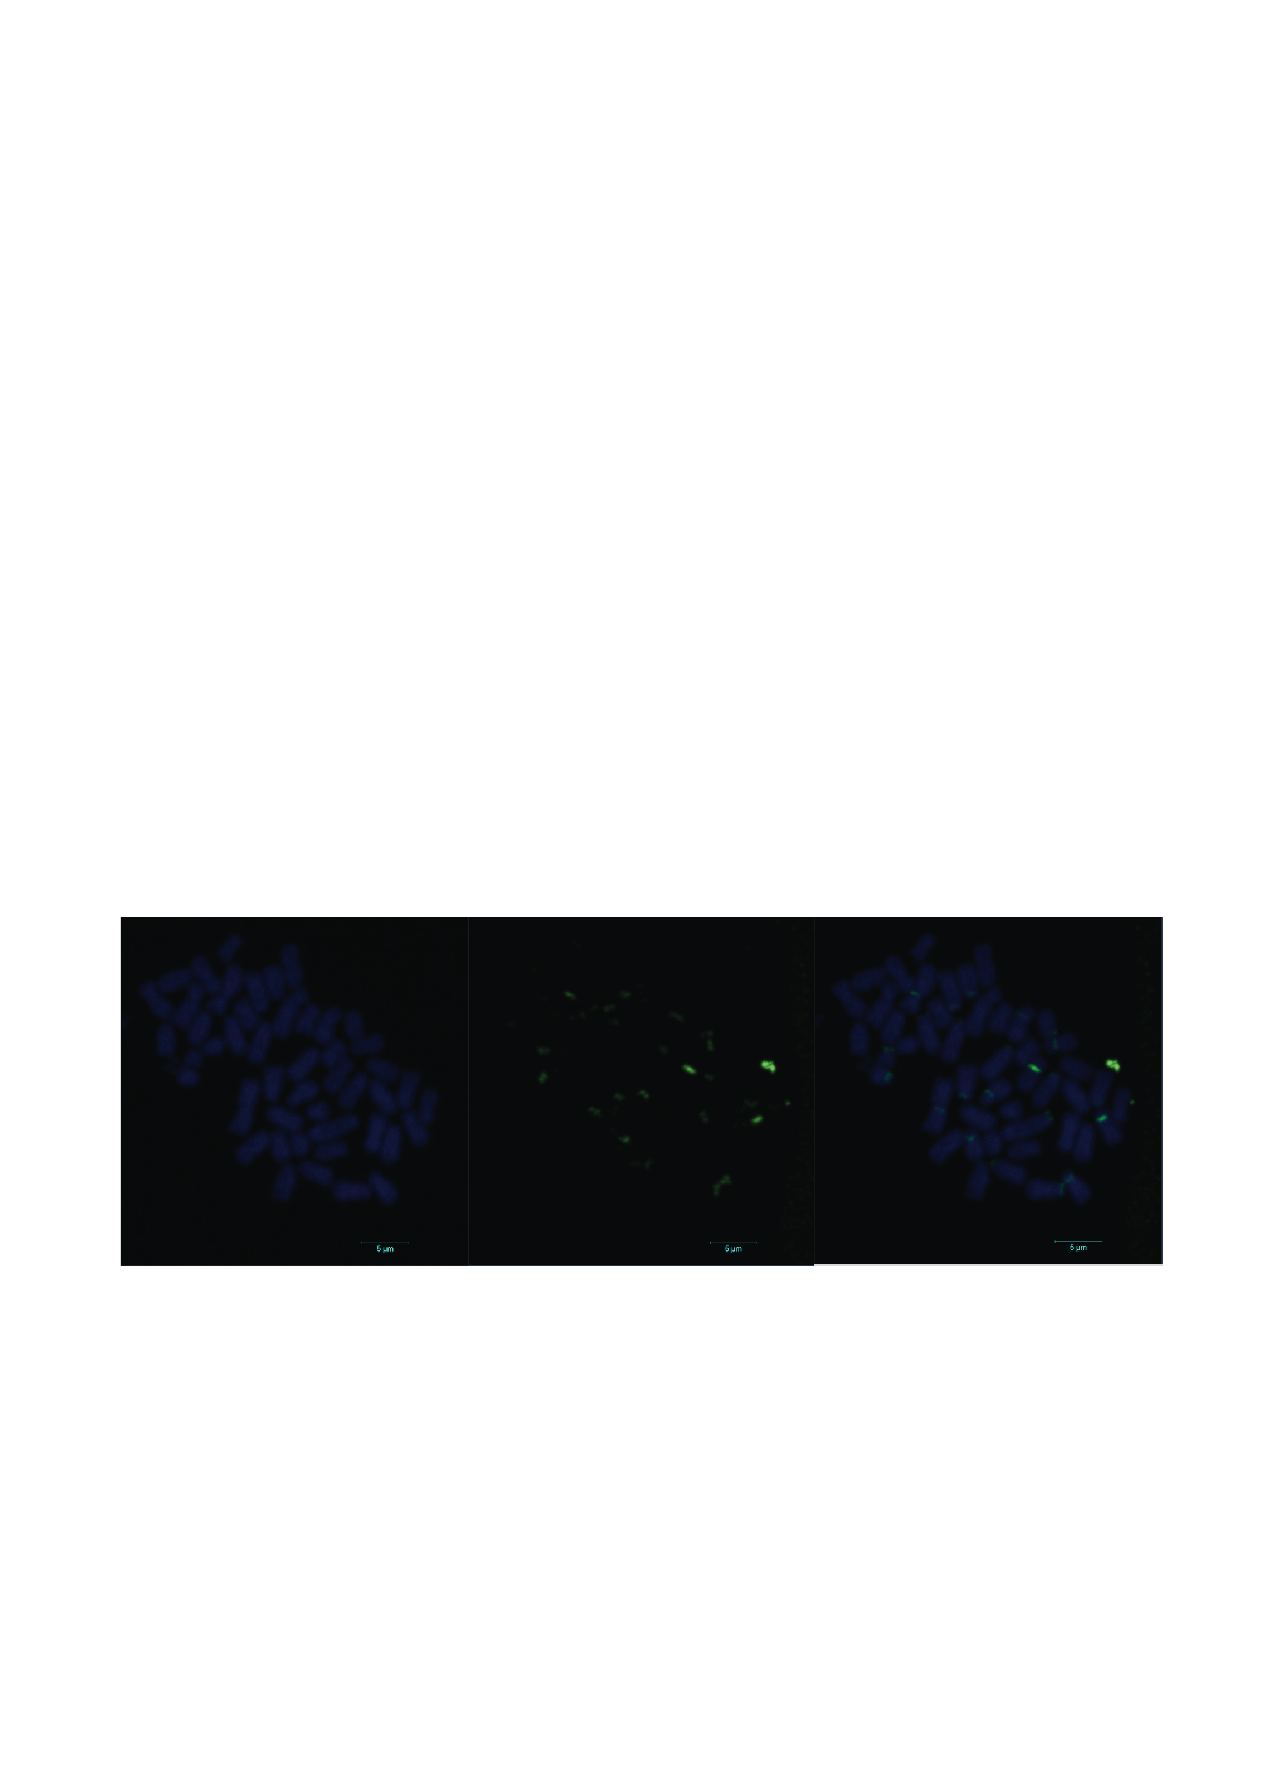
\includegraphics[width=\linewidth]{fish_all_probes.pdf}
    \caption{
      The candidate centromeric satellite sequence and three derivative sequences localized to the centromeres of $\sim$13 pairs of chromosomes. (left) DNA is stained with DAPI. (center) probes are stained green. (right) two images are combined.
    }
    \label{fish_all}
  \end{figure*}


\subsection*{Validation of centromeric sequence assembly}
  The repetitive nature of centromeric sequences inevitably accompanies the possibility of misassembly. Although long-range assembly correctness on the assembled genomes was verified with BAC-end and fosmid-end reads and Hi-C contact frequency data, exact sequence ordering within long centromeric repeat arrays can be inaccurate. In order to validate the centromeric sequence assembly, PacBio raw subreads were mapped to the assembled genomes and read coverage over centromeric regions was visualized for manual inspection.

  PacBio subread were mapped to the medaka genomes by BLASR \cite{Chaisson2012} with a strict mapping parameters (see Methods). The assembly validity was then manually inspected on the genomic browser by confirming that enough number of subreads covered the centromeric repeat arrays without breaks. Most part of the centromeric sequences were covered by enough number of subreads, although a small number of exceptions were observed in chromosomes 9, 13 and 20 in the Hd-rR genome, which contained one or two breaking points that were not spanned by subreads (Fig.\,\ref{centromere_landscape}). Although the assembly validation using somewhat erroneous PacBio reads cannot completely exclude the possibility of misassembly, indeed long-range ordering over the centromeric repeat arrays can be inaccurate, nevertheless relatively narrow range of assembly can be ascertained and that is adequately informative for observing sequence composition of a specific chromosome or inter-chromosomal sequence similarity.


\subsection*{Inter-chromosomal centromeric sequence conservation}
  It is widely known that in some species centromeric sequences exhibit inter-chromosomal conservation that are considered to derive from evolutionary rearrangements of chromosomes and/or frequent sequence exchange as a result of co-localization in the nucleus \cite{Willard1991}. In order to reveal the presence of inter-chromosomal relationship of centromeric repeats in the medaka genomes, satellite sequences from each chromosome were compared.

  Centromeric repeat arrays in each chromosome were decomposed into satellite monomers by RepeatMasker and the monomers were clustered by DNACLUST \cite{Ghodsi2011} with $>$85\% sequence similarity threshold. For those clusters that have $\geq$10 members, the monomer with the longest sequence in the cluster was chosen as the representative monomer of the cluster. All-vs-all pairwise alignment of the representative monomers from each chromosome along with the representative monomer identified by Melters \textit{et al}. was performed and pairwise distance was calculated. Based on this distance, hierarchical clustering of the chromosome-representative monomers were performed. The chromosome-representative monomers were clustered into four groups, revealing the presence of super-chromosomal subfamilies (Fig.\,\ref{monomer_clustering}, Table\,\ref{super_chromosomal_subfamily}). Many (15 out of 24) chromosomes (chr.\,2, 3, 5, 6, 7, 10, 11, 12, 14, 15, 16, 18, 20, 22 and 23) were assigned exclusively to one of the four subfamilies. Five chromosomes (chr.\,1, 4, 8, 13 and 19) were clustered into two or three subfamilies but significantly more monomers were classified to one subfamily over the others, thus they are assigned to the dominant subfamily. Chromosomes 9 and 21 were classified into two subfamilies with no significant preference. Chromosomes 17 and 24 could not be classified due to the lack or insufficient amount of centromeric repeats in either of the three assembled genomes. Overall, 22 out of 24 chromosomes were assigned to one or two subfamilies.

  Intriguingly, each subfamily exhibited distinct preference of centromeric positions in chromosomes; namely subfamily (SF) 2 for acrocentric, SF 1 and 3 for submetacentric and subtelocentric and SF 4 for metacentric, respectively (Table \ref{super_chromosomal_subfamily}). This tendency is analogous to the traditional observation that human acrocentric chromosomes share highly identical alpha-satellite sequences \cite{Willard1991}.

  In those chromosomes that had sufficient amount of centromeric repeats in multiple strains, most (7 out of 9) chromosomes were classified into the same subfamilies among strains. One of the exceptions was chromosome 19, where representative monomers from Hd-rR and HSOK were classified into SF 1 while that of HNI into SF 3, although the repeats from each strain were confirmed to locate in close position of the chromosome as they were flanked by a corresponding pair of genetic markers (Fig.\,\ref{fig:repeat_distribution}). This discordant classification may be because the assemblies of each strain captured different subregion of the corresponding repeat arrays or due to misassembly in one or more strains. The other exception was chromosome 21, where the representative monomers from the acrocentric array of Hd-rR were classified into SF 2, those from the metacentric array of Hd-rR and from the acrocentric array of HNI into SF 3. The two acrocentric arrays from Hd-rR and HNI were located at close but distinct positions in the chromosome (Fig.\,\ref{fig:repeat_distribution}), thus it may well contain different repeat sequence profiles and be classified into different subfamilies. The overall conservation of centromeric satellites among the three strains which separated 18 and 25 million years ago is in line with the previous observation that centromeric sequences were conserved among species within about 50 million years after separation \cite{Melters2013}.

  \begin{figure*}
    \centering
    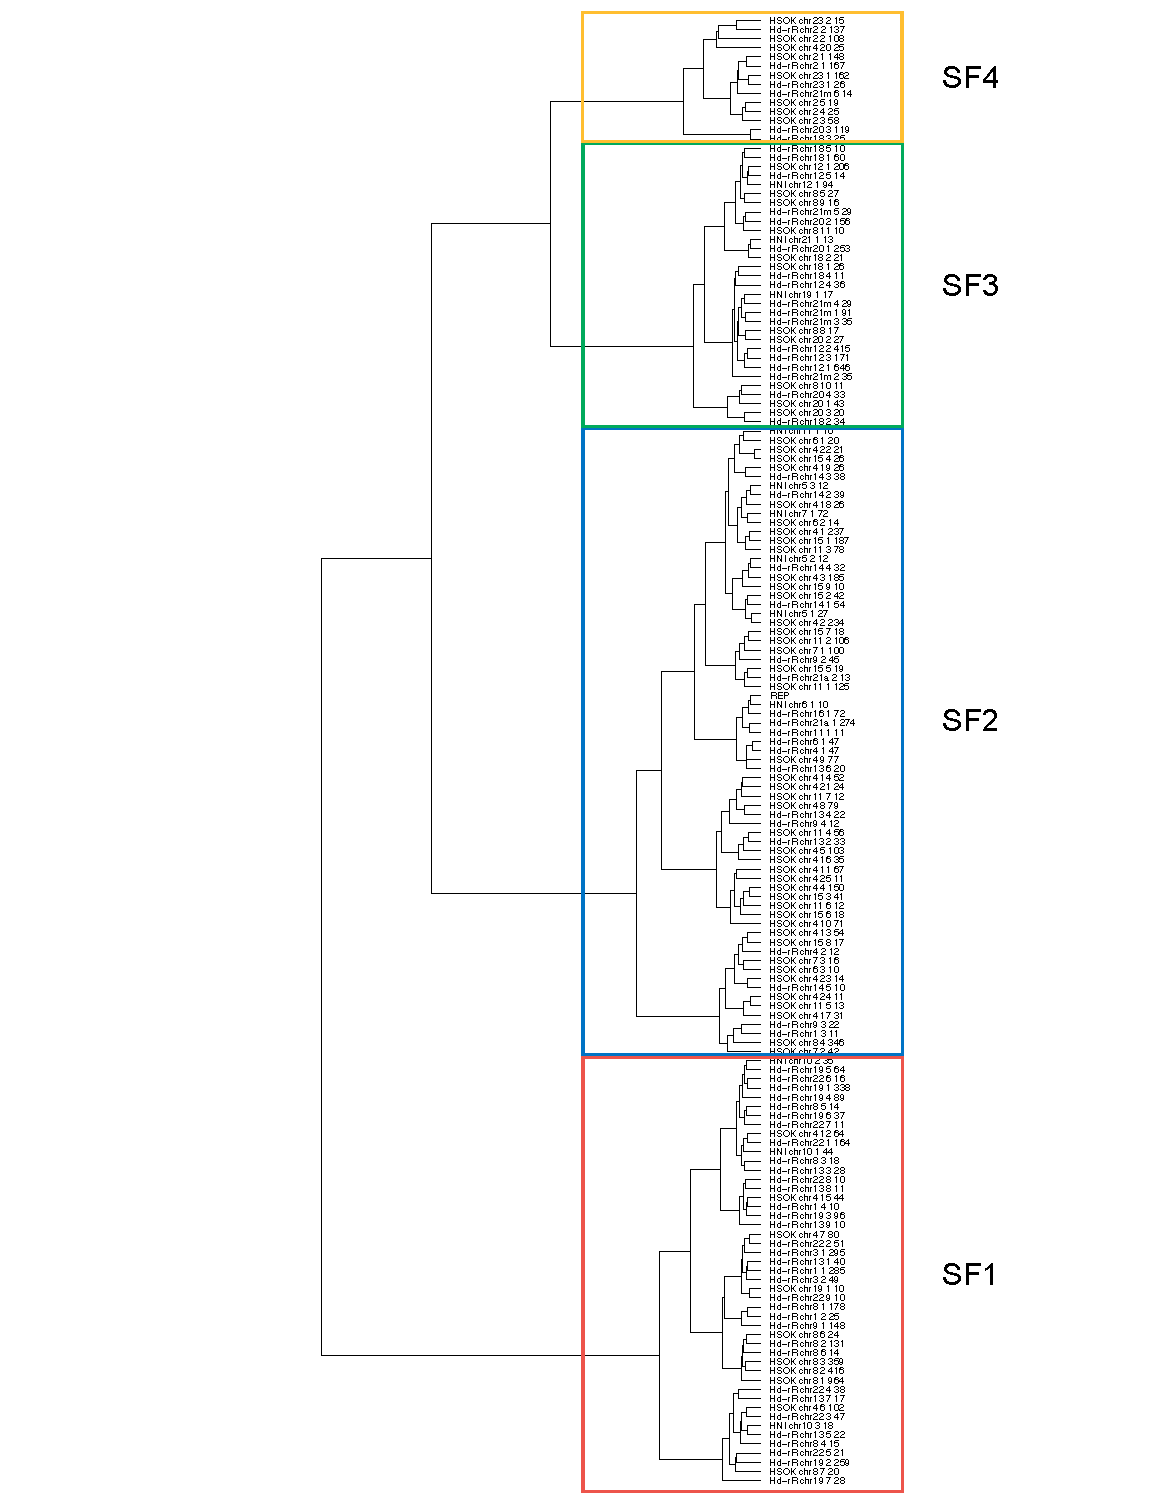
\includegraphics[width=\linewidth]{monomers_clustering.pdf}
    \caption{
      Hierarchical clustering of chromosome-representative monomers. Monomers are labeled as species, chromosome, cluster index, number of the cluster constituents. The clustering revealed four large subfamilies of satellite monomers.
    }
    \label{monomer_clustering}
  \end{figure*}

  \begin{table*}
    \centering
    \caption{Super-chromosomal subfamilies of centromeric repeats}
    \begin{tabular}{p{0.6cm}p{3.4cm}p{1.5cm}p{2cm}p{4.5cm}p{3.7cm}}
  \hline
  SF & Hd-rR & HNI & HSOK & combined & positions \\ \hline
  1 & 4,6,9,11,14,16,21a (1,13) & 5,6,7,11    & 4,6,7,11,15 (8) & 4,5,6,7,9,11,14,15,16,21a (1,8,13) & 1M+1SM+14A (2SM+1A) \\
  2 & 1,3,8,9,13,19,22          & 10          & 8,19 (4)        & 1,3,8,9,10,13,19,22 (4)            & 6SM+2ST+2A (1M) \\
  3 & 12,18,20,21m (8)          & 12,21 (19)  & 12,18,20 (8)    & 12,18,20,21m (8,19)                & 1M+8SM+2ST+1A (2SM) \\
  4 & 2,23 (21m)                &             & 2,23 (4)        & 2,23 (4,21m)                       & 3M+1SM (2M) \\
  \hline
\end{tabular}

    \label{super_chromosomal_subfamily}
    \caption*{{\small
      Chromosomes were classified into four subfamilies (SF). Chromosomes in brackets are the ones that have significantly more amount of repeats classified into another subfamily. Hd-rR chromosome 21 possessed two distantly-positioned arrays, thus is notated as 21m (metacentric) and 21a (acrocentric; see Table \ref{centromeric_repeat_distribution} for detail). Summarizing the chromosomes from the three strains, 22 out of the 24 chromosomes were assigned to one or two subfamilies. Notation of the centromeric positions are the same as Table \ref{centromeric_repeat_distribution}.
    }}
  \end{table*}


\subsection*{Sequence organization at the centromeres}
  Sequence organization on the assembled centromeric sequences were analyzed. Self-alignment dot plots of the centromeric sequences on each chromosome are shown in Supplementary Figure \ref{centromere_landscape}.

  HSOK chromosome 8 captured the longest centromeric arrays, namely two arrays of 250\,kb and 95\,kb flanking an assembly gap (Fig.\,\ref{chr8_browser}A). These two arrays were comprised of the satellites from three subfamilies (SF\,1, SF\,2, SF\,3). SF\,1 satellites comprise large inner portion of the arrays, interspersed by SF\,2 satellites; these sequences were flanked by smaller amount of SF\,3 satellites. Multiple alignment of the chromosome-representative monomers revealed that the representative monomer of the forth largest cluster which belongs to SF\,2 possessed $\sim$10-bp insertion compared to the representative monomers belonging to SF\,1, yet otherwise looks nearly identical (Fig.\,\ref{chr8_multiple_alignment}). The assignment of these representative monomers to the different subfamilies was due to the definition of the distance used for the hierarchical clustering, which was calculated by alignment identity of two sequences and thus large indels cause substantial loss in the identity. On the other hand, the representative monomers belonging to SF\,3 exhibit distinct sequence composition from the monomers in SF\,1 and SF\,2. Interestingly, the orientation of the satellite sequences switched at the boundaries of SF\,1 and SF\,3 arrays (Fig.\,\ref{chr8_browser}A). This suggests the scenario that the SF\,1 array inserted into the SF\,3 array as a result of a sequence conversion, unequal crossover or other chromosome rearrangement events. Switches of sequence orientation in satellite arrays have also been observed in the pericentromeric regions of human chromosomes \cite{M.KatharineRuddand2004}. Overall similar sequence organization was observed in the same chromosome of Hd-rR, which had 20-kb and 40-kb SF\,1 arrays flanking an assembly gap and a 1-kb SF\,3 array at the outside of the 20-kb SF\,1 array (Fig.\,\ref{chr8_browser}B).

  Another interesting example was HSOK chromosome 4 which captured a over 300-kb nearly continuous array (Fig.\,\ref{chr4_browser}). This array was comprised mainly of SF\,2 satellites, interspersed with shorter SF\,1 satellite arrays. Also small amount of SF\,4 satellites were observed in downstream portion. Furthermore, frequent switches of sequence orientation were observed, some of which correspond to the SF boundaries whereas others do not.

  Chromosome 12 was the only chromosome that all the three strain genomes captured $>$10-kb centromeric arrays. The Hd-rR assembly reached the centromeric region from the both sides; HNI reached from the p-arm side; HSOK reached from the q-arm side (Fig.\,\ref{chr12_transition}A). All the arrays were comprised of SF\,3 satellites. In order to examine if the sequences of these centromeric transition regions are conserved among the strains, dot plots were drawn (Fig.\,\ref{chr12_transition}B,\,C). Whereas modest sequence conservation was observed in the surrounding unique regions, apparent conservation of the sequence structure, including linear ordering of the satellites, was not conserved. Similar unconservation of the sequence ordering in centromeric transition regions were observed in some other chromosomes (Fig.\,\ref{other_chroms_transition}). These results imply that the centromeric repeat arrays have evolved rapidly compared to the other genomic region, in line with traditional observations \cite{Willard1991}.

  The self-alignment dot plots revealed the presence of higher-order repeats (HORs) in many chromosomes (Fig.\,\ref{centromere_landscape}). The HORs observed here seem somewhat diverged, unlike highly-identical HORs observed in the core centromeric regions of human and some other primates \cite{Willard1987}. This is, however, reasonable because a stretch of highly-identical HOR array longer than the PacBio read length ($\sim$50\,kb at maximum) would fail to be assembled. Therefore, the absence of highly-homogenized HORs in the assembled sequences does not exclude the possibility of the presence of them in inner centromeric regions in medaka. Moreover, the fact that all the contigs containing the centromeric repeats were truncated in the middle of the centromeric arrays implies the presence of highly-homogenized sequences.


  \begin{figure*}
    \centering
    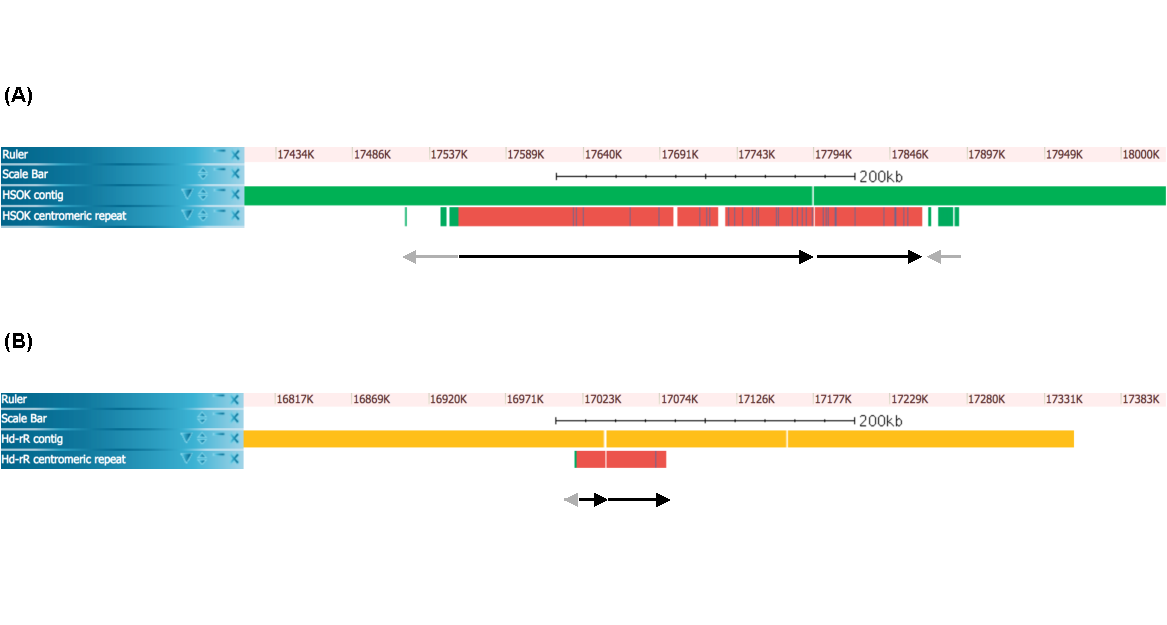
\includegraphics[width=\linewidth]{chr8_browser.pdf}
    \caption{
      Sequence organization of chromosome 8 centromeric regions. (A) HSOK chromosome 8 had 250-kb and 95-kb repeat arrays flanking an assembly gap. SF\,1 satellites (red) comprise large inner portion of the arrays, interspersed by SF\,2 satellites (blue). These sequences were flanked by shorter SF\,3 satellite arrays (green). The orientation of the satellite sequences switched at the boundaries of SF\,1 and SF\,3 arrays (indicated by black and grey arrows). (B) Hd-rR had similar sequence organization as HSOK.
    }
    \label{chr8_browser}
  \end{figure*}

  \begin{figure*}
    \centering
    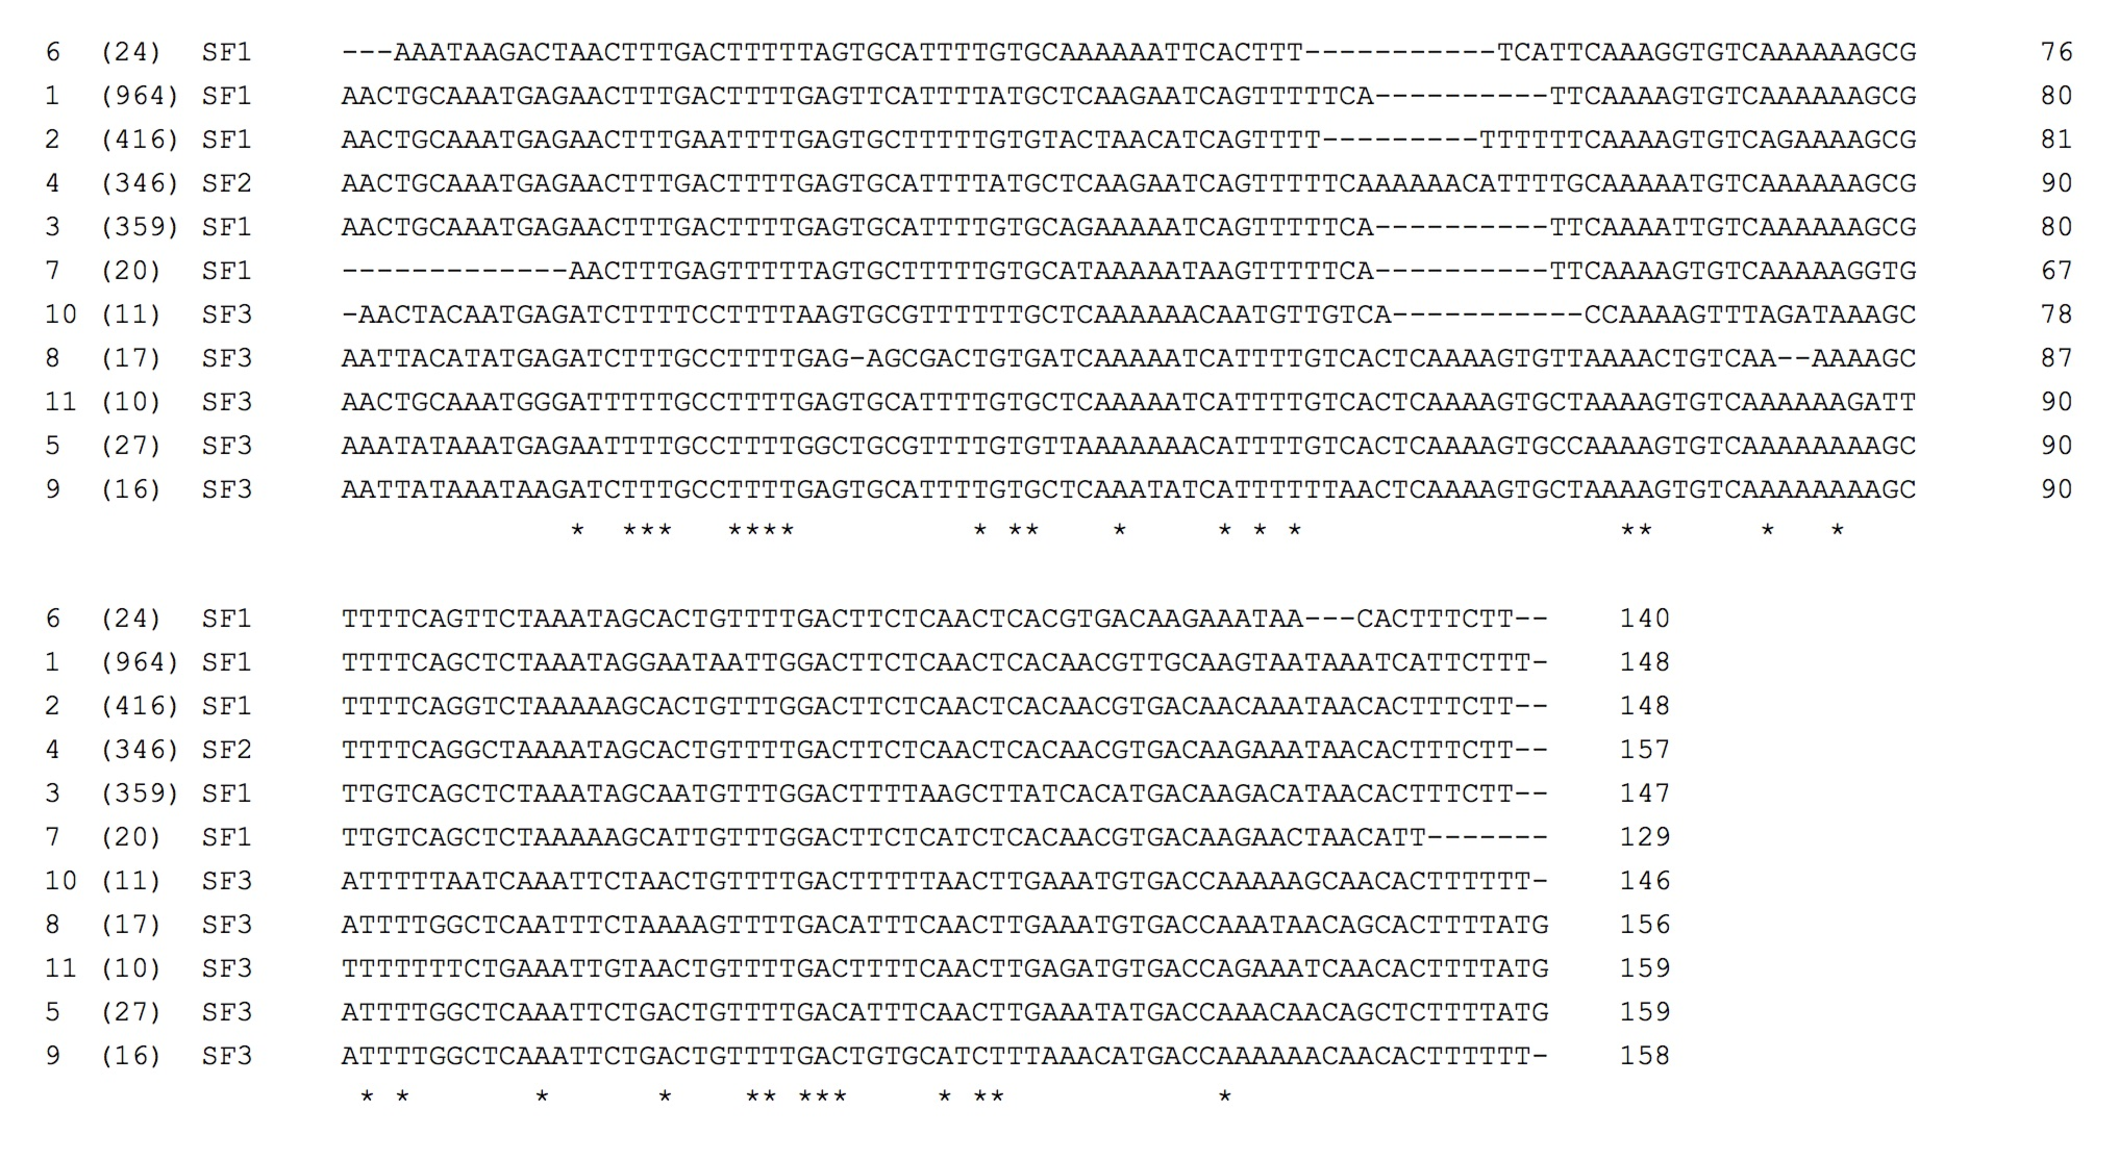
\includegraphics[width=\linewidth]{chr8_multiple_alignment.pdf}
    \caption{
      Multiple sequence alignment of HSOK chromosome 8 representative monomers. 11 representative monomers of HSOK chromosome 8 were aligned using Clustal Omega (version 1.2.3) \cite{Sievers2011}. The labels of each sequence represent cluster index (as a descending order of cluster size), number of monomers belonging to the cluster (in brackets) and belonging subfamilies. Asterisks ("*") indicate the nucleotides shared in all the representative monomers. Representative monomer 4 which belongs to SF\,2 has $\sim$10-bp insertion compared to SF\,1 representative monomers, yet otherwise shares virtually the same sequence composition. SF\,3 representative monomers have distinct sequence composition from SF\1, and SF\2 representative monomers.
    }
    \label{chr8_multiple_alignment}
  \end{figure*}

  \begin{figure*}
    \centering
    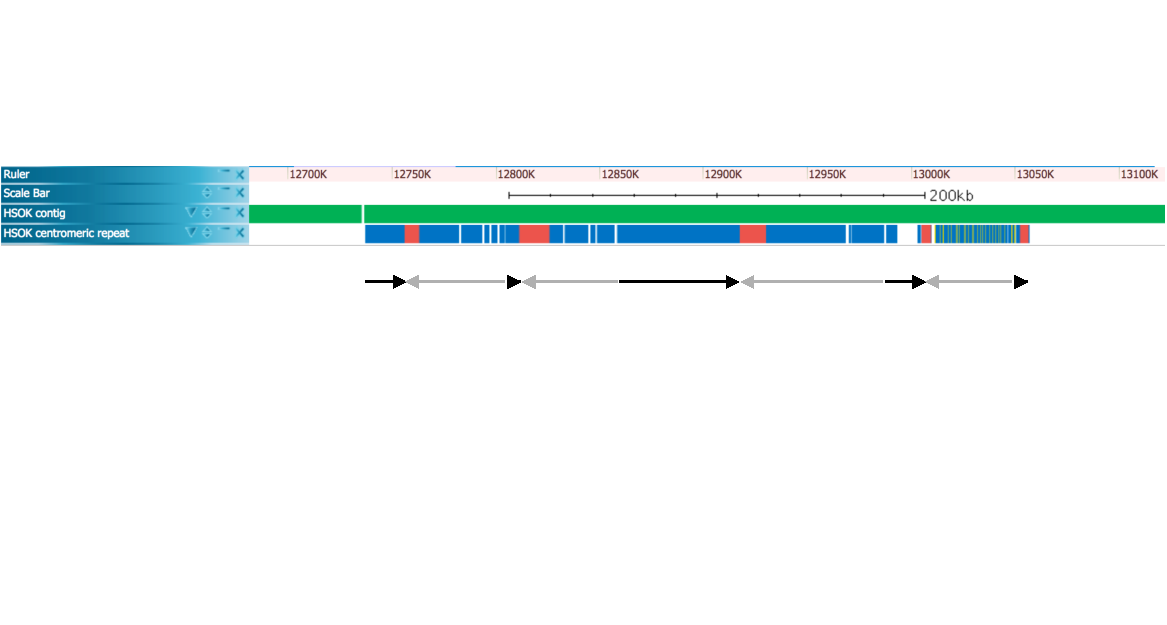
\includegraphics[width=\linewidth]{chr4_browser.pdf}
    \caption{
      Sequence organization of HSOK chromosome 4 centromeric region. The $\sim$300-kb nearly continuous array was truncated by the contig end at the left end. The array was comprised mainly of SF\,2 satellites (blue) and these are interspersed by shorter SF\,1 satellite arrays (red). Also small amount of SF\,4 satellites (yellow) were observed in the right portion. Frequent switches of sequence orientation were observed (indicated by black and grey arrows).
    }
    \label{chr4_browser}
  \end{figure*}

  \begin{figure*}
    \centering
    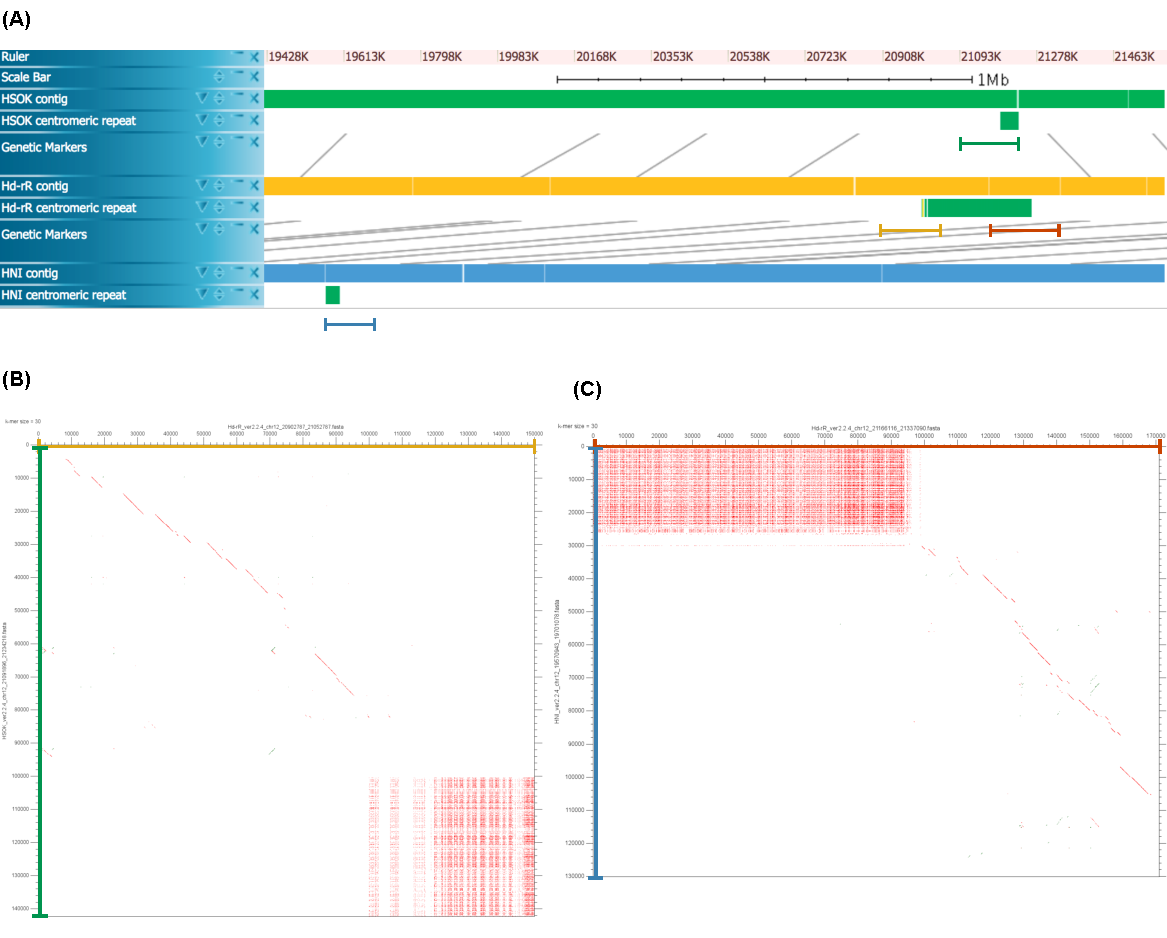
\includegraphics[width=\linewidth]{chr12_transition.pdf}
    \caption{
      Comparison of the centromeric transition regions of chromosome 12. (A) The Hd-rR assembly reached the centromeric region from the both sides (separated by a contig gap); HNI reached from the p-arm side; HSOK reached from the q-arm side. The grey lines indicate the positions of corresponding genetic markers. (B) Sequences of the q-arm transition regions of Hd-rR and HSOK was compared. (C) Sequences of the p-arm transition regions of Hd-rR and HNI was compared. Dots represent 30-bp exact matches between two sequences. Whereas modest conservation was observed in the surrounding unique sequences (indicated by the chained diagonal lines), no clear conservation was observed within the centromeric array sequences.
    }
    \label{chr12_transition}
  \end{figure*}


\section*{Discussion}
Due to the long-standing difficulty in assembling repetitive DNA, in-depth analyses of centromeric sequences have been limited \cite{Plohl2014}. Based on the high-quality genomes of the three medaka inbred strains which were recently assembled with PacBio long reads, this study has conducted a comprehensive analysis of the centromeric sequences in medaka. This is, to the author's knowledge, the first in-depth study of centromeric sequence organization in fish species.

This study has revealed the presence of four subfamilies of the centromeric satellites. The satellites of each subfamily are possessed by generally different subset of chromosomes. The presence of centromeric satellite subfamilies have been also observed in human, in which, similarly to the medaka satellite subfamilies, each subfamily belongs to generally different subsets of chromosomes \cite{Alexandrov2001}. Although 22 out of the 24 chromosomes were classified to one or two subfamilies, the classification could be imperfect. This is because many chromosomes have relatively short repeat arrays in the assemblies which locate at the ends of much larger original arrays and the peripheral regions tend to accumulate mutations \cite{Smith1976, Schueler2001}.

It was also observed that the subfamilies had different preference for the centromeric positions in chromosomes. For example, the medaka SF\,2 showed clear preference for acrocentric chromosomes. This is analogous to the human acrocentric chromosomes (chr.\,13, 14, 21 and 22) which share highly identical alpha-satellites \cite{Willard1991}. The human acrocentric chromosomes possess nucleolus organizers region (NOR) at their short arms and are present in close proximity in the nucleolus, where frequent sequence exchange are believed to occur \cite{Willard1991}. Although the presence of NORs have not been investigated in this study, the same mechanism may work in medaka and produce the high centromeric sequence similarity in the acrocentric chromosomes. It is uncertain if any biological mechanism works for the concerted centromeric positions in the other subfamilies; or they might just be the ``remnants'' that are left after collecting the acrocentric chromosomes.

This study has also revealed the conservation of centromeric satellites among the three strains which are estimated to have separated 18 (Hd-rR and HNI) and 25 (HSOK and the previous two) million years ago (MYA) \cite{Setiamarga2009}. This conservation is consistent with a previous comparative study of 282 animal and plant species that observed the centromeric satellites are conserved among species within 50 million years after separation \cite{Melters2013}, whereas unconserved centromeric repeat as a result of rapid diversification has also been observed in some closely-related species \cite{Lee2005}. It has been known that the teleost lineage underwent a whole-genome duplication (WGD) 336--404 MYA and since that medaka has largely retained the genomic structure without major chromosome rearrangements \cite{Kasahara2007}. The inter-chromosomal centromeric sequence comparison in this study have shown that the chromosome pairs that derived from the WGD do not necessarily possess similar centromeric satellite sequences. Combined with the Melters \textit{et al.}'s observation, it can be speculated that medaka centromeric sequences have massively diverged since the WGD. Furthermore, the sequence organization including linear ordering of satellites were not conserved among the strains, suggesting that the centromeric sequences have evolved independently after the strain separations.

The medaka genome assemblies using PacBio long reads captured centromeric arrays in many chromosomes, including some long arrays over 100 kb. However the amount of centromeric repeats identified in the contigs that were anchored to the chromosomes was substantially below the estimated genomic abundance of the centromeric repeats in all the strains. Indeed large amount of the repeats were found in unanchored contigs. BAC/fosmid-end reads and Hi-C contact frequency data were used for the Hd-rR genome assembly, which successfully anchored a number of contigs containing centromeric repeats and resulted in higher portion of centromeric repeats to be anchored despite shorter read length than HSOK. This result emphasizes the complementary power of other long-range information methods in addition to the long read sequencing. The sum of the centromeric repeats in anchored and unanchored contigs did not reach the estimated genomic abundance, suggesting uncertain amount of the repeats were lost in the assembly process. Highly-homogenized HORs which might exist in the inner centromeric regions may have caused the under-represtation of centromeric repeats in the assembled contigs.

The centromeric sequence organization of three medaka strains revealed in this study provides insights into centromeric sequence evolution. Also, the characterized centromeric sequences provides a important basis for understanding the possible contribution of DNA sequences to the centromere specification and function.


\section*{Methods}
\subsection*{Genome assembly}
  Assembly of the three medaka strain genomes were carried out by Kazuki Ichikawa and Jun Yoshimura in the same laboratory. The detail of the methods will be described in Ichikawa \textit{et al}. (unpublished). Here a brief overview of the methods is described.

  The genomes were sequenced with PacBio RSII sequencer and were assembled into contigs with FALCON assembler \cite{Chin2016}. The contigs were then polished with PacBio reads using Quiver \cite{Chin2013} and with Illumina reads using Pilon \cite{Walker2014}. A number of contigs that contained long centromeric repeat arrays were not polished with Pilon because it was observed that extremely more bases were corrected on centromeric regions than other genomic regions presumably due to mismapping of short reads. The polished contigs were mapped to the chromosomes using SNP genetic markers. Hd-rR contigs were further scaffolded using BAC- and fosmid-end pair reads. Also a number of unanchored contigs were positioned into the chromosomes using Hi-C contact frequency data.


\subsection*{Validation of centromeric sequence assembly}
  PacBio raw subreads were mapped to the assembled genomes by BLASR (version 5.2.6fa6cc2) \cite{Chaisson2012} with parameters of ``{-}{-}bestn 10 {-}{-}minReadLength 10000 {-}{-}minSubreadLength 10000 {-}{-}minAlnLength 5000 {-}{-}minPctSimilarity 80''. Then the mapped subreads that have $>$85\% sequence identity in the 1-kb sequences at the both alignment ends were selected and visualized on the genomic browser. The centromeric repeat regions were manually inspected and confirmed that they were covered by enough number of overlapping subreads (at least 5 subreads and typically much more reads at every position) without breaks (Fig.\,\ref{centromere_landscape}).


\subsection*{Estimation of genomic abundance of centromeric repeats}
  In order to minimize the effect of high error rate of PacBio sequencing on abundance estimation of the centromeric repeats, only high quality subreads were used for this step. Specifically, subreads were filtered with the criteria that average base quality over the all bases $>$10. Also, subreads shorter than 1 kb were excluded. The filtered subreads were then scanned by RepeatMasker (version 4.0.6) \cite{Smit} with sensitive setting using the medaka representative centromeric satellite monomer sequence as a custom library. Genomic fraction of the medaka centromeric satellite for each strain was estimated by the ratio of total amount of masked centromeric satellite in the total length of the filtered subreads (Table \ref{centromeric_repeat_genomic_abundance}).


\subsection*{Identification of centromeric repeats in the genomes and classification of centromeric positions}
  The three medaka strain genomes were searched for the medaka centromeric satellite by RepeatMasker with sensitive setting. For those chromosomes that have $>$1 kb centromeric repeat, positions of the centromeres were classified employing the nomenclature defined in Levan \textit{et al.} \cite{levan1964}. The nomenclature divides a chromosome equally into eight portions and classify the chromosome by the position of the centromere from the two most inners to the two most outers as metacentric, submetacentric, subtelocentric and acrocentric. In this study, chromosomes were classified into a portion that contains the largest amount of centromeric repeats.


\subsection*{Designing FISH probe sequences}
  The candidate centromeric satelilte identified by Melters \textit{et al.} \cite{Melters2013} was first used as a FISH probe but hybridized to only 5$\sim$7 pairs of chromosomes. Subsequently, additional probe sequences were designed as follows. For each chromosome, satellite monomers were collected from satellite arrays and the collected monomers were aligned back to the original array with BLASTN (in BLAST+ suite, version 2.3.0)\cite{Camacho2009}. Then a monomer with the highest score was chosen as the representative monomer of the chromosome, where the score was defined as:

  \[
    score = \sum_{\mbox{hits}} \mbox{alignment identity} \cdot \frac{\mbox{alignment length}}{\mbox{query length}}.
  \]

  Representative monomers obtained from each chromosome were then aligned to the Hd-rR genome with BLASTN and three monomers that exhibited high identity to different subsets of chromosomes were chosen as additional probe sequences (Fig.\,\ref{fish_each}).


\subsection*{FISH experiments}
  The FISH experiments were carried out by Yusuke Inoue at the Department of Biological Sciences, Graduate School of Science, The University of Tokyo.

  Centromeric satellite DNA were synthesized by annealing and extension of two DNA oligos using TaKaRa ExTaq (TaKaRa), followed by subcloning into pCR\texttrademark II-TOPO\textregistered vector (Thermo). DNA probes were prepared by cutting and labeling the plasmid DNA with biotin, using Nick Translation Kit (Roche). Medaka fibroblast cells were treated with 0.05 $\mu$g/ml of corcemid (for probe1,2) or 1 $\mu$M of nocodazole (for probe3, 4, all) for 4--5 hours. After trypsinization, cells were hypotonically swollen in 75mM KCl for 20 minutes, fixed with ice-cold Carnoy's solution (1:3 acetic acid: methanol), then spread onto slides. After RNase treatment and denaturation of chromosomal DNA, hybridization was carried out by dropping probe DNA solution onto slides and incubating at 37\,\celsius\, for overnight. After washing, chromosomal DNA was incubated with avidin-FITC (Vector Laboratories) for 1 hour. After final wash, slides were mounted with Vectashield Plus DAPI (Vector Laboratories). Images were acquired using a fluorescence microscope (LSM710, Zeiss).


\subsection*{Selection of chromosome-representative monomers and hierarchical clustering}
  Centromeric repeat arrays in each chromosome of the three strains were decomposed into satellite monomers by RepeatMasker. The monomer sequences within each chromosome were then clustered into groups of $>$85\% sequence similarity by DNACLUST \cite{Ghodsi2011} (parameters: ``-d -l -s 0.85 {-}{-}no-k-mer-filter''). For those clusters that have $\geq$10 members, the monomer with the longest sequence in the cluster was chosen as the representative monomer of the cluster. All-vs-all pairwise alignment of the chromosome-representative monomers along with the representative monomer identified by Melters \textit{et al.} \cite{Melters2013} was performed by needle program in EMBOSS suite (version 6.5.7) \cite{Rice2000}. The distance between a pair of two monomers was calculated as below:

  \[
    \mbox{distance} = 1 - \frac{\mbox{number of matched bases}}{\mbox{length of shorter monomer}}
  \]

  Based on this distance, hierarchical clustering of the chromosome-representative monomers were performed by "hclust" function in R (version 3.2.4) with "ward.D2" method.


\section*{Acknowledgements}
The author would like to thank Professor Shinichi Morishita for guiding my research work, Yuta Suzuki, Yuichi Motai, Yoshihiko Suzuki, Kazuki Ichikawa, Jun Yoshimura and other laboratory members, Hiroyuki Takeda, Ryohei Nakamura, Masahiko Kumagai and Yusuke Inoue (in the Takeda laboratory at the Department of Biological Sciences, Graduate School of Science, The University of Tokyo) for valuable discussion, advice and supports.


%% References
\begin{small}
\ja{
\bibliographystyle{bib/myunsrt}
\bibliography{bib/master}
}
\end{small}

%% Supplements
\onecolumn
\beginsupplement
\section*{Supplements}
\begin{table}[htbp]
  \centering
  \caption{PacBio sequencing statistics}
  \begin{tabular}{lccc}
  \hline
  & Hd-rR & HNI & HSOK \\ \hline
  Number of cells & 38 (P6-C4) + 35 (P5-C3) + 78 (P4-C2) & 24 (P5-C3) + 144 (P4-C2)	& 97 (P6-C4) \\
  Number of filtered subreads & 13,359,879	& 14,777,797 & 5,527,528 \\
  Total bases (bp) & 87,095,247,396 & 52,830,178,508 & 60,649,832,062 \\
  Average read length (bp) & 6,519 & 3,575 & 10,972 \\
  \hline
\end{tabular}

  \label{sequencing_stats}
\end{table}

\begin{table}[htbp]
  \centering
  \caption{Centromeric repeat genomic abundance}
  \begin{tabular}{p{1.5cm}p{2.5cm}p{3cm}p{3cm}p{3.5cm}p{2.5cm}}
  \hline
  strain & total subreads & passed subreads & passed subreads & repeats in passed subreads & estimated genomic abundance \\ \hline
  Hd-rR & 13,359,879 & 4,586,550 (34.33\%) & 34,933,754,979 bp & 354,930,731 bp (1.02\%) &  8.13 Mb \\
  HNI   & 14,777,797 & 7,265,969 (49.17\%) & 28,478,925,597 bp & 338,807,989 bp (1.19\%) &  9.52 Mb \\
  HSOK  &  5,527,528 & 1,955,979 (35.39\%) & 23,106,352,588 bp & 460,716,149 bp (1.99\%) & 15.95 Mb \\
  \hline
\end{tabular}

% \begin{tabulary}{18cm}{LRRRRR}
%   \hline
%   strain & total subreads & passed subreads & passed subreads & repeats in passed subreads & estimated genomic abundance \\ \hline
%   Hd-rR & 13,359,879 & 4,586,550 (34.33\%) & 34,933,754,979 bp & 354,930,731 bp (1.02\%) &  8.13 Mb \\
%   HNI   & 14,777,797 & 7,265,969 (49.17\%) & 28,478,925,597 bp & 338,807,989 bp (1.19\%) &  9.52 Mb \\
%   HSOK  &  5,527,528 & 1,955,979 (35.39\%) & 23,106,352,588 bp & 460,716,149 bp (1.99\%) & 15.95 Mb \\
%   \hline
% \end{tabulary}

  \label{centromeric_repeat_genomic_abundance}
\end{table}

%% Centromeric repeat distribution
\begin{figure}[p]
  \centering
  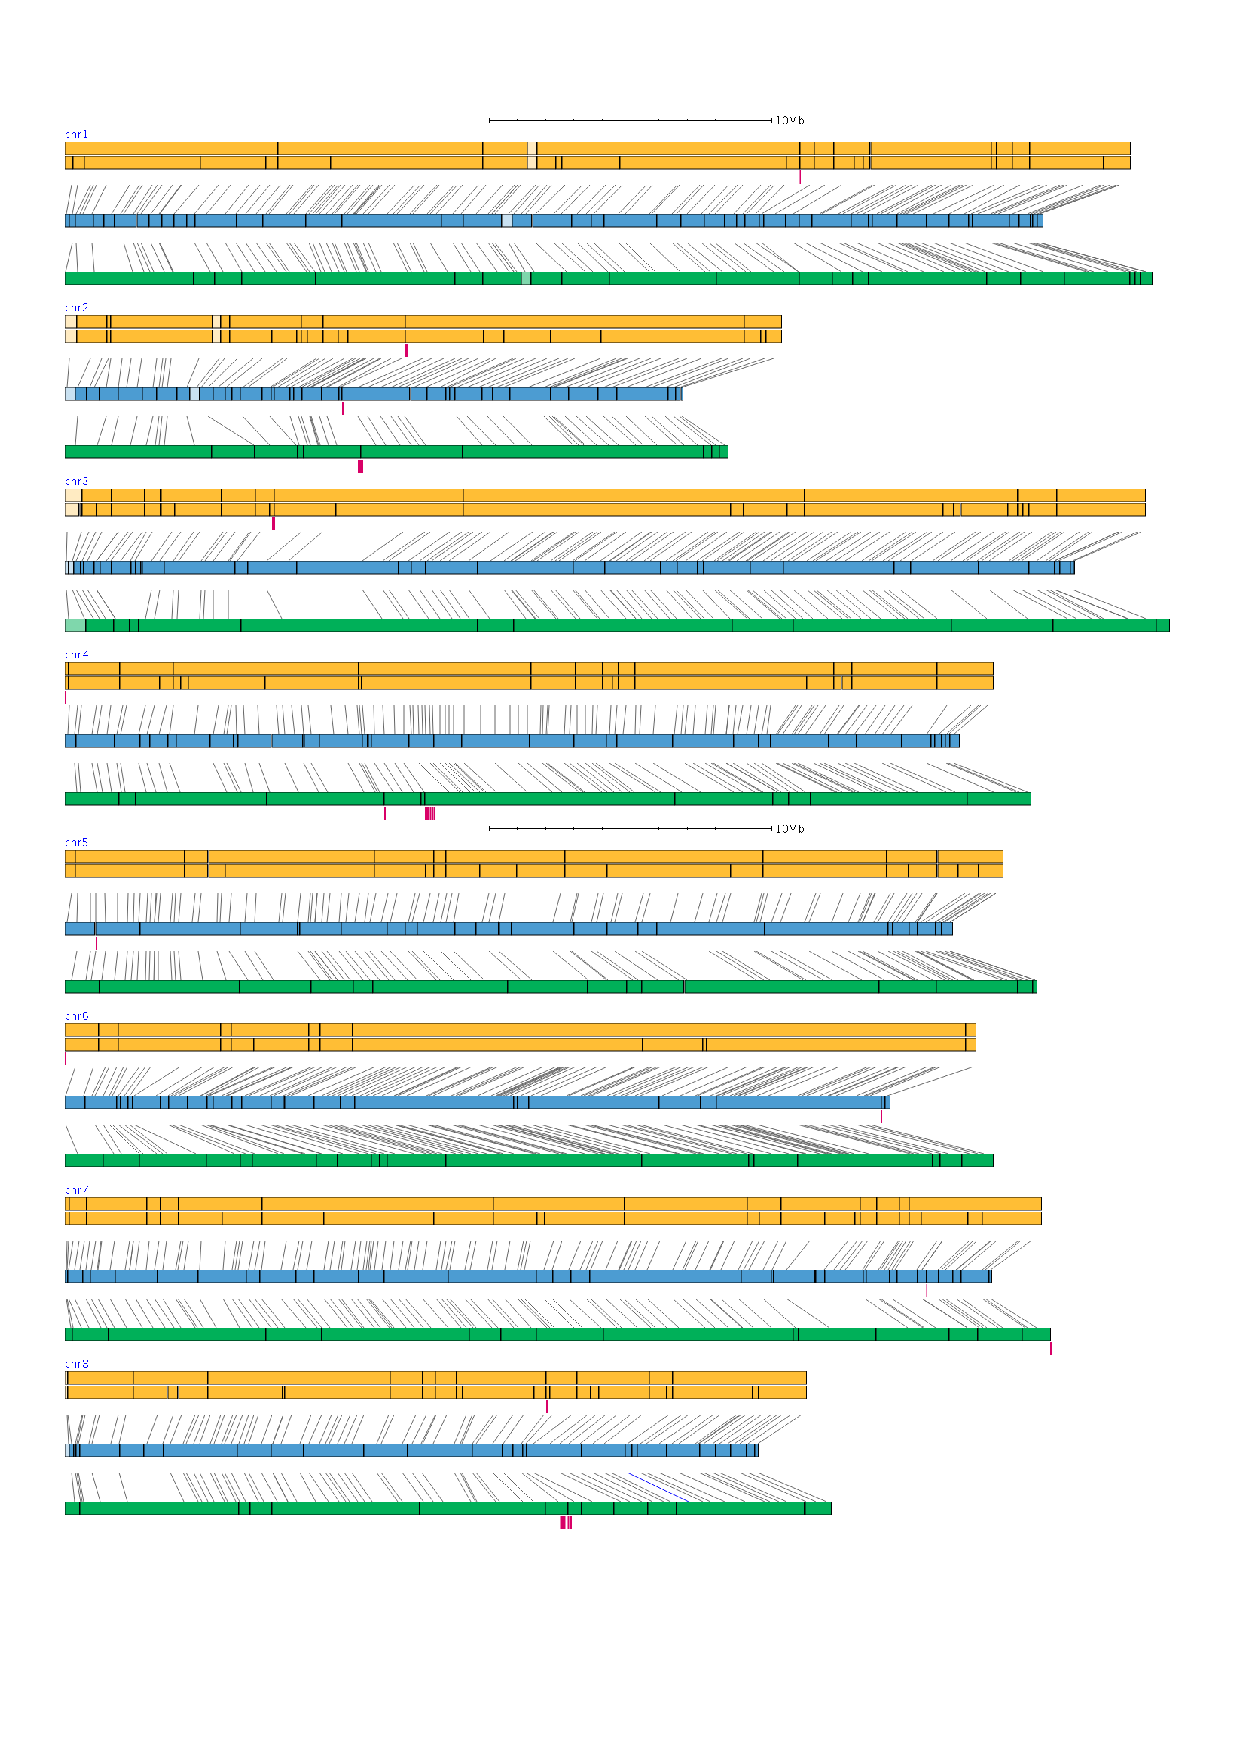
\includegraphics[width=\linewidth]{repeat_distribution_1.pdf}
  \caption{
    Centromeric repeat distribution. Yellow, Hd-rR scaffolds (upper) and contigs (lower); blue, HNI contigs; green, HSOK contigs; red, centromeric repeats; grey, corresponding genetic markers.
  }
  \label{fig:repeat_distribution}
\end{figure}

\addtocounter{figure}{-1}
\begin{figure}[p]
  \centering
  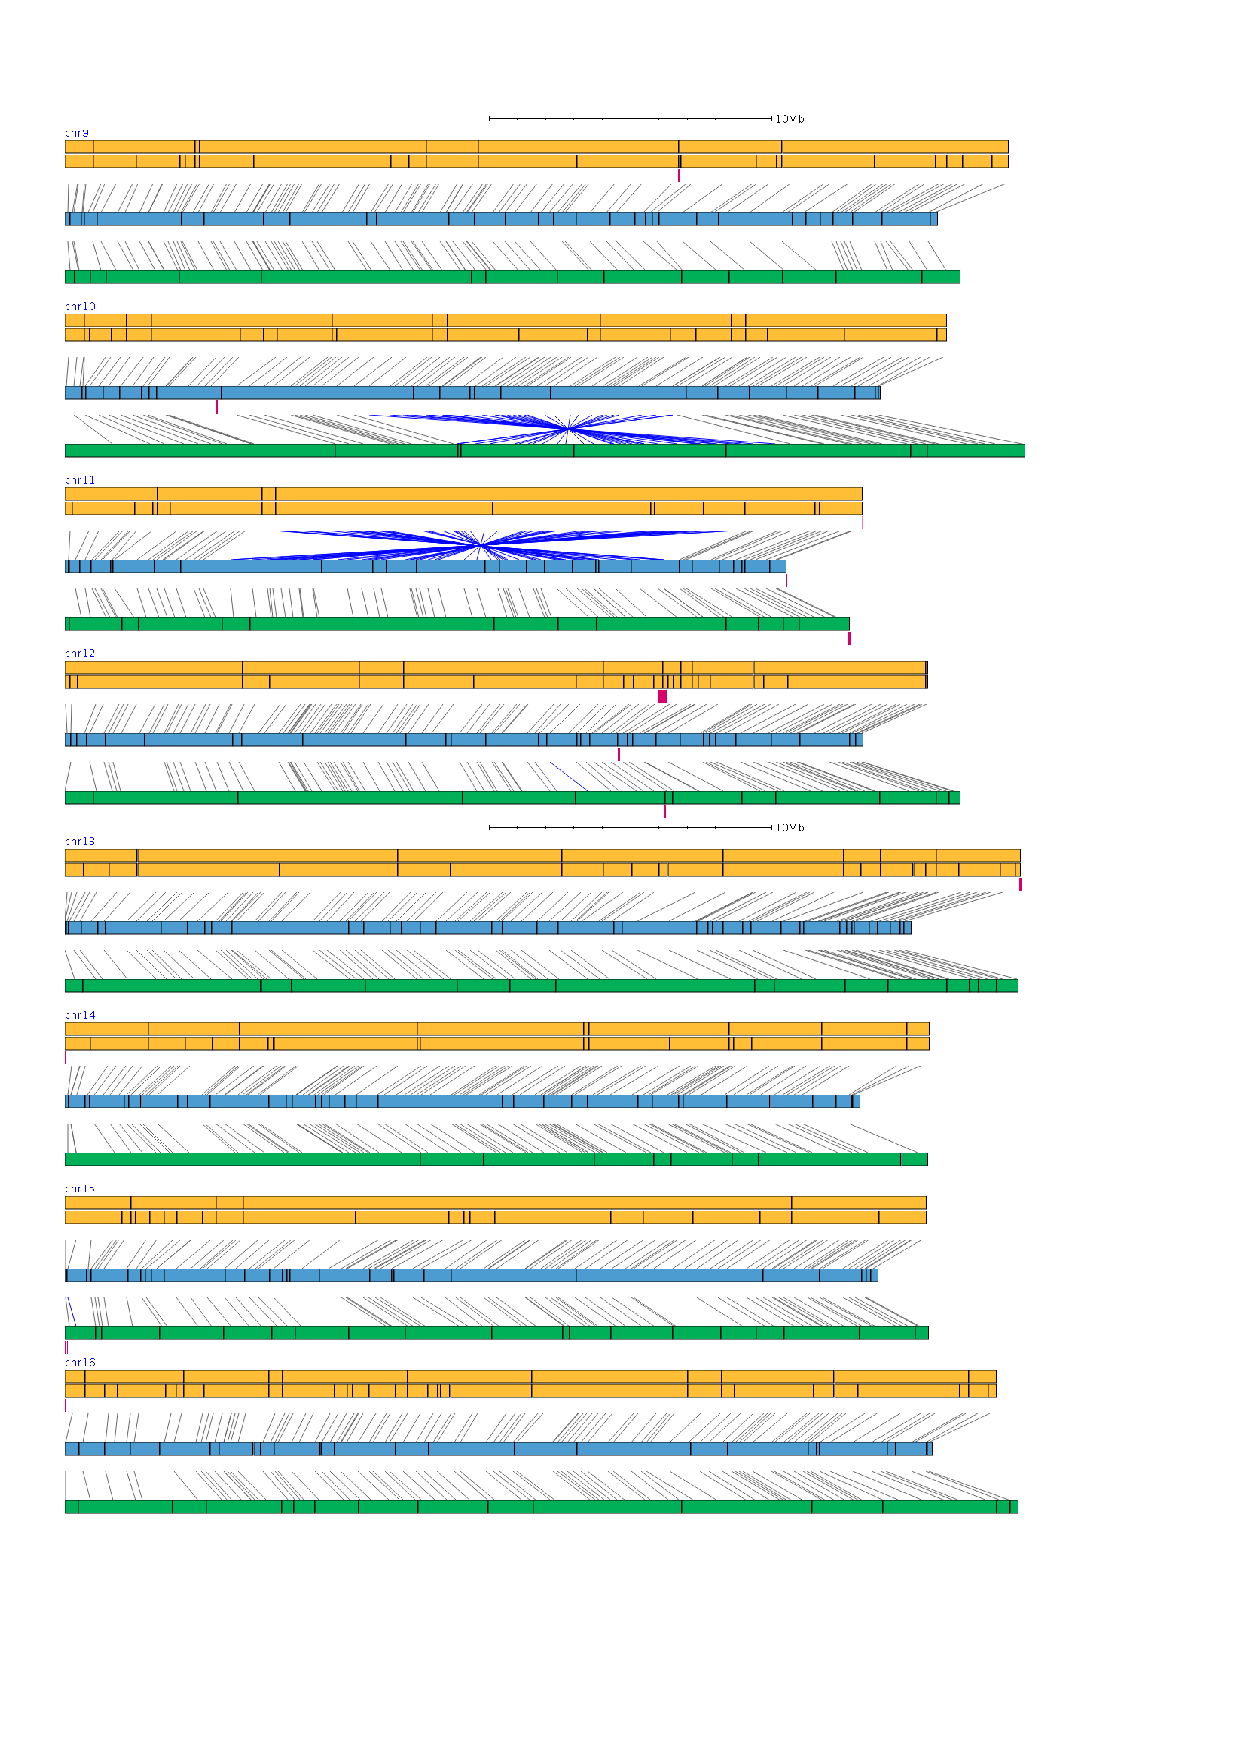
\includegraphics[width=\linewidth]{repeat_distribution_2.pdf}
  \caption{
    Centromeric repeat distribution. Yellow, Hd-rR scaffolds (upper) and contigs (lower); blue, HNI contigs; green, HSOK contigs; red, centromeric repeats; grey, corresponding genetic markers.
  }
  \label{fig:repeat_distribution}
\end{figure}

\addtocounter{figure}{-1}
\begin{figure}[p]
  \centering
  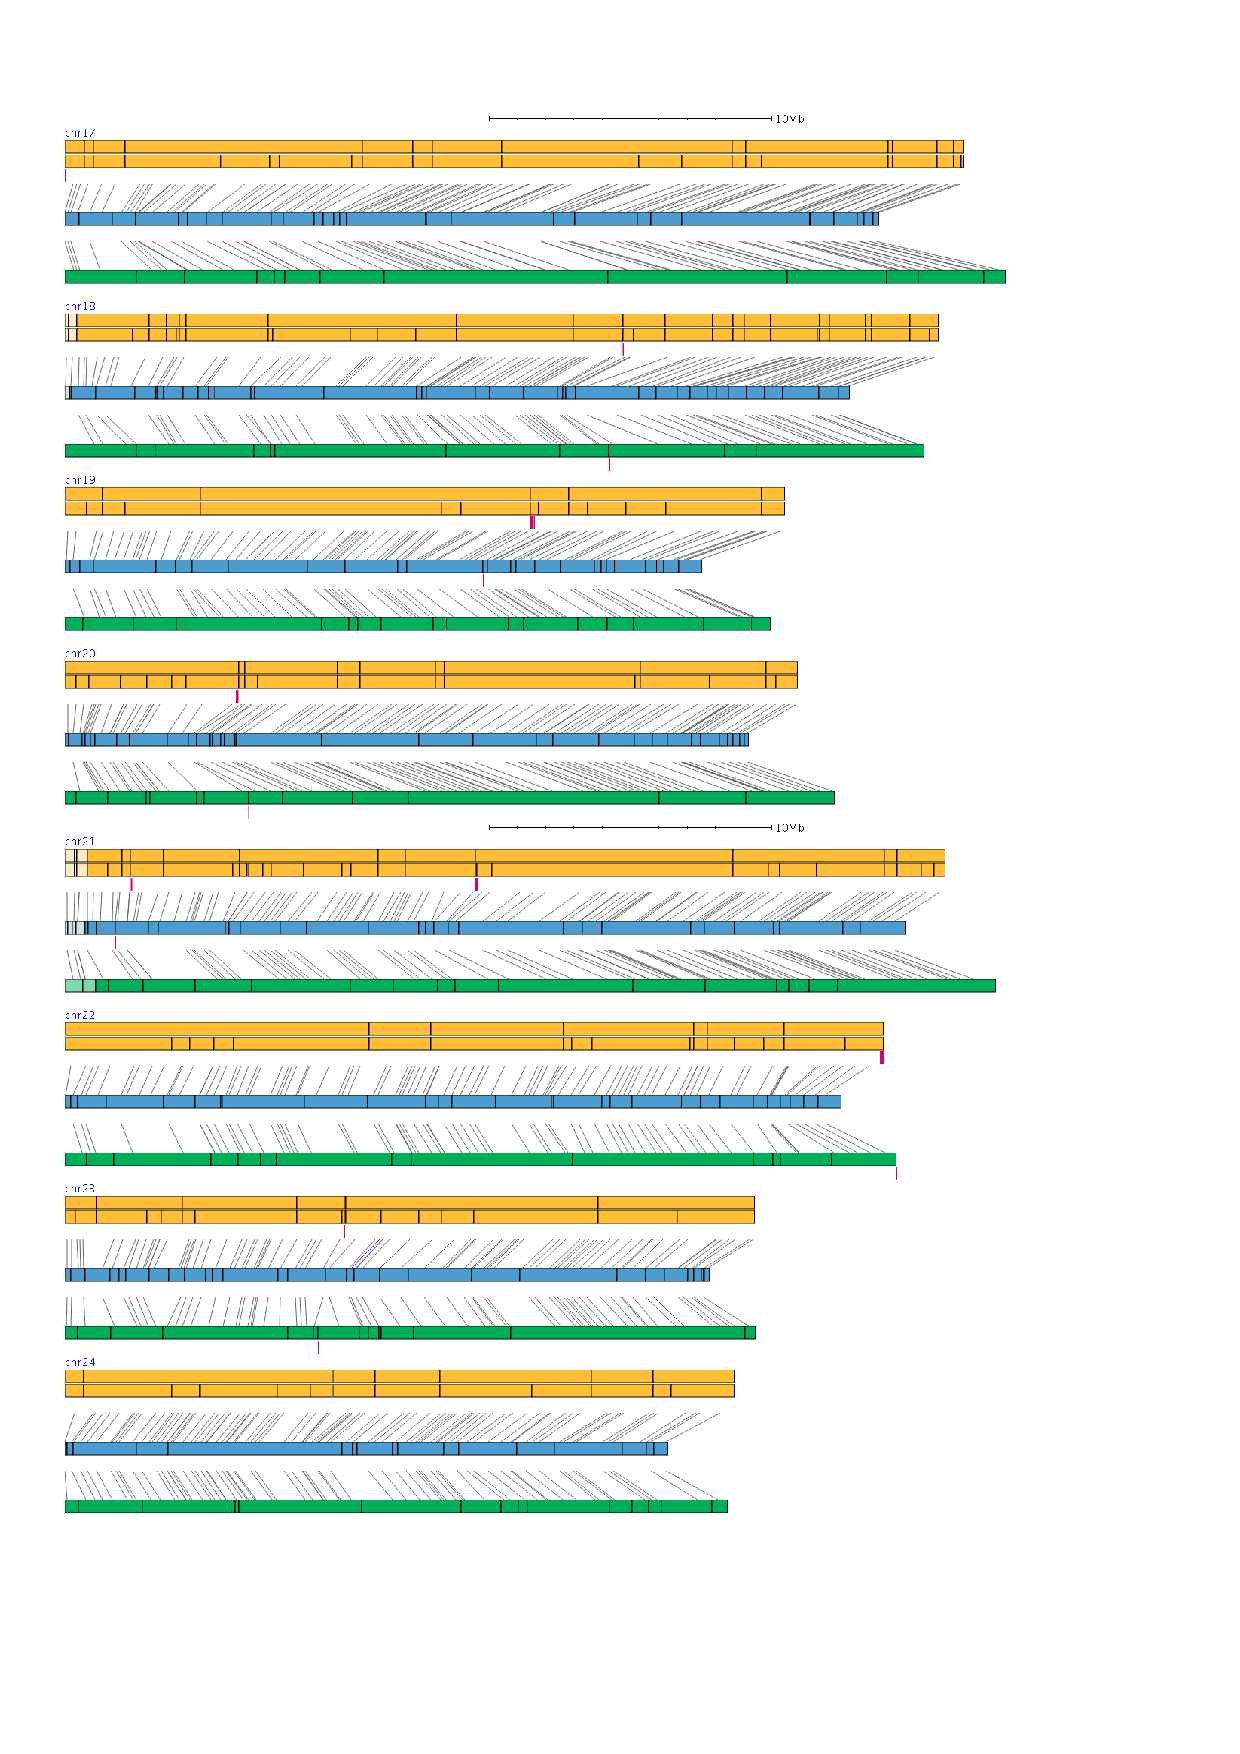
\includegraphics[width=\linewidth]{repeat_distribution_3.pdf}
  \caption{
    Centromeric repeat distribution. Yellow, Hd-rR scaffolds (upper) and contigs (lower); blue, HNI contigs; green, HSOK contigs; red, centromeric repeats; grey, corresponding genetic markers.
  }
  \label{fig:repeat_distribution}
\end{figure}



\begin{figure}[p]
  \centering
  %\includegraphics{}
  \caption{
    Centromere landscapes in the medaka genomes
  }
  \label{centromere_landscape}
\end{figure}

\begin{figure}[p]
  \centering
  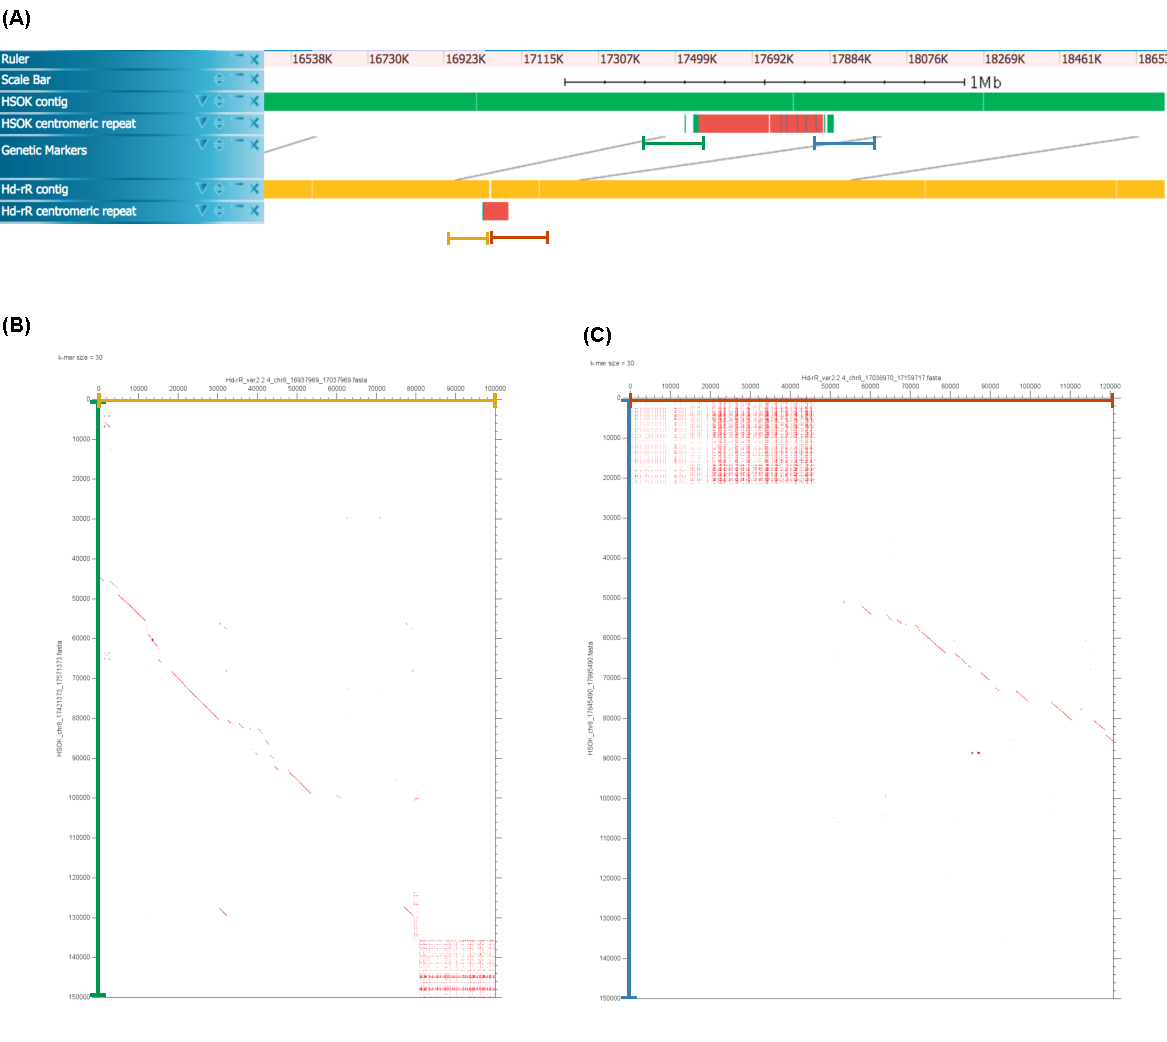
\includegraphics[width=\linewidth]{chr8_transition.pdf}
  \caption{
    (A, B, C) Comparison of the centromeric transitional regions of chromosome 8 of Hd-rR and HSOK.
  }
  \label{other_chroms_transition}
\end{figure}

\addtocounter{figure}{-1}
\begin{figure}[p]
  \centering
  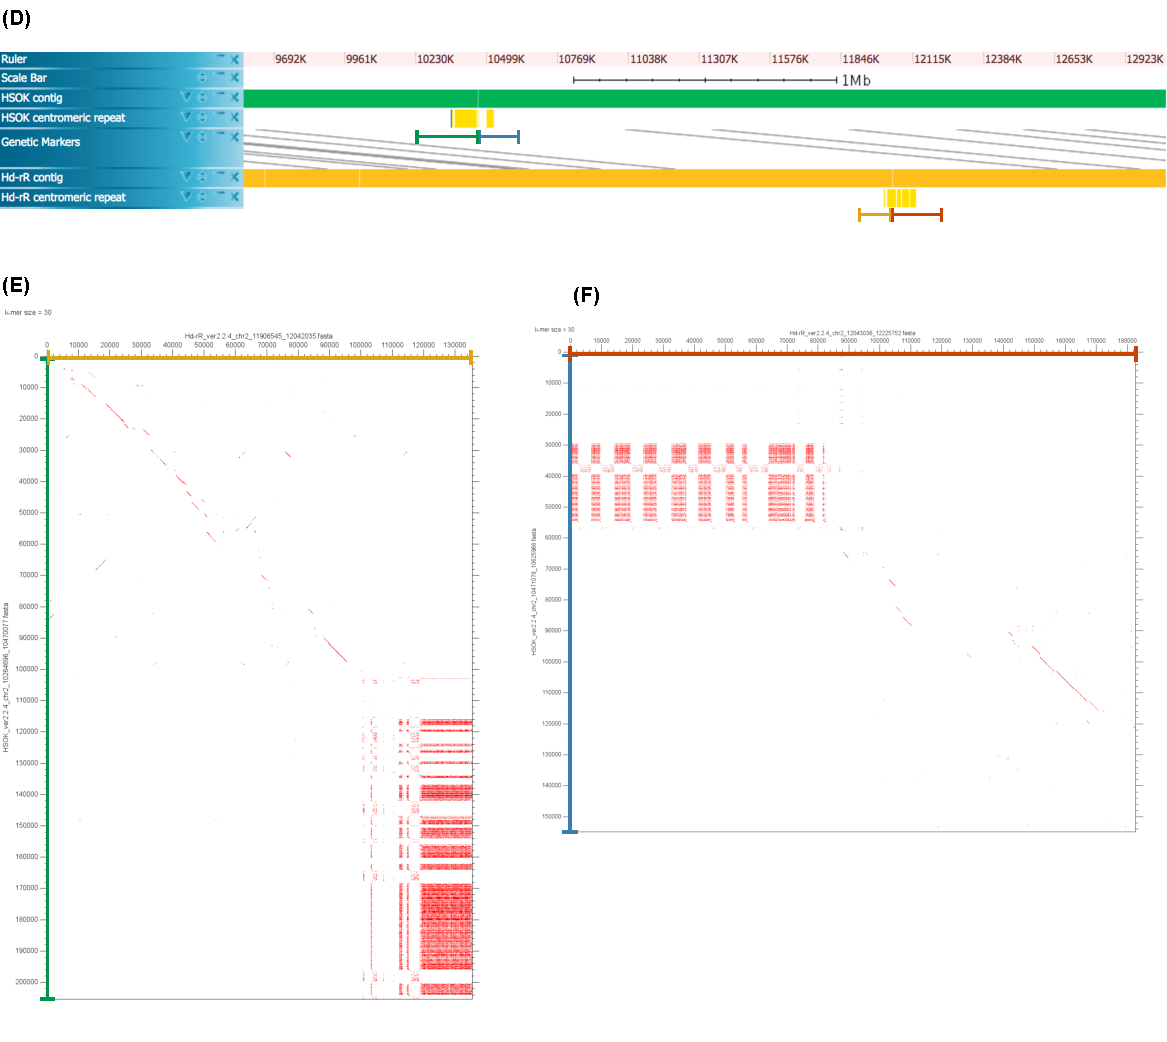
\includegraphics[width=\linewidth]{chr2_transition.pdf}
  \caption{
    (D, E, F) Comparison of the centromeric transitional regions of chromosome 2 of Hd-rR and HSOK.
  }
\end{figure}


\end{document}
